% !TeX spellcheck = hu_HU
% !TeX encoding = UTF-8
% !TeX program = xelatex

\documentclass[11pt,a4paper,oneside]{report}             % Single-side
%\documentclass[11pt,a4paper,twoside,openright]{report}  % Duplex

% thanks to http://tex.stackexchange.com/a/47579/71109
\usepackage{ifxetex}
\usepackage{ifluatex}
\newif\ifxetexorluatex % a new conditional starts as false
\ifnum 0\ifxetex 1\fi\ifluatex 1\fi>0
   \xetexorluatextrue
\fi

\ifxetexorluatex
  \usepackage{fontspec}
\else
  \usepackage[T1]{fontenc}
  \usepackage[utf8]{inputenc}
  \usepackage[lighttt]{lmodern}
\fi

\usepackage[english,magyar]{babel} % Alapértelmezés szerint utoljára definiált nyelv lesz aktív, de később külön beállítjuk az aktív nyelvet.

%\usepackage{cmap}
\usepackage{amsfonts,amsmath,amssymb} % Mathematical symbols.
%\usepackage[ruled,boxed,resetcount,linesnumbered]{algorithm2e} % For pseudocodes. % beware: this is not compatible with LuaLaTeX, see http://tex.stackexchange.com/questions/34814/lualatex-and-algorithm2e
\usepackage{booktabs} % For publication quality tables for LaTeX
\usepackage{graphicx}

%\usepackage{fancyhdr}
%\usepackage{lastpage}

\usepackage{anysize}
%\usepackage{sectsty}
\usepackage{setspace} % For setting line spacing

\usepackage[unicode]{hyperref} % For hyperlinks in the generated document.
\usepackage{xcolor}
\usepackage{listings} % For source code snippets.

\usepackage[amsmath,thmmarks]{ntheorem} % Theorem-like environments.

\usepackage[hang]{caption}

\singlespacing

\newcommand{\selecthungarian}{
	\selectlanguage{magyar}
	\setlength{\parindent}{2em}
	\setlength{\parskip}{0.5em}
	\renewcommand{\baselinestretch}{1.0}
%	\frenchspacing
}

\newcommand{\selectenglish}{
	\selectlanguage{english}
	\setlength{\parindent}{0em}
	\setlength{\parskip}{0.5em}
	\nonfrenchspacing
	\renewcommand{\figureautorefname}{Figure}
	\renewcommand{\tableautorefname}{Table}
	\renewcommand{\partautorefname}{Part}
	\renewcommand{\chapterautorefname}{Chapter}
	\renewcommand{\sectionautorefname}{Section}
	\renewcommand{\subsectionautorefname}{Section}
	\renewcommand{\subsubsectionautorefname}{Section}
}

\usepackage[numbers]{natbib}
\usepackage{xspace}


%TODO Set the main variables
\newcommand{\vikszerzoVezeteknev}{Zalavári}
\newcommand{\vikszerzoKeresztnev}{Márton}

\newcommand{\vikkonzulensAMegszolitas}{dr.~}
\newcommand{\vikkonzulensAVezeteknev}{Friedl}
\newcommand{\vikkonzulensAKeresztnev}{Katalin}

\newcommand{\vikkonzulensBMegszolitas}{}
\newcommand{\vikkonzulensBVezeteknev}{}
\newcommand{\vikkonzulensBKeresztnev}{}

\newcommand{\vikkonzulensCMegszolitas}{}
\newcommand{\vikkonzulensCVezeteknev}{}
\newcommand{\vikkonzulensCKeresztnev}{}

\newcommand{\vikcim}{Módszerek közel optimális vágások keresésére} % Cím
\newcommand{\viktanszek}{\bmeszit} % Tanszék
\newcommand{\vikdoktipus}{\msc} % Dokumentum típusa (\bsc vagy \msc)
\newcommand{\vikmunkatipusat}{diplomatervet} % a "hallgató nyilatkozat" részhez: szakdolgozatot vagy diplomatervet

%--------------------------------------------------------------------------------------
% TDK-specifikus változók
%--------------------------------------------------------------------------------------
%\newcommand{\tdkszerzoB}{Második Szerző} % Második szerző neve; hagyd üresen, ha egyedül írtad a TDK-t.
\newcommand{\tdkev}{2021} % A dolgozat írásának éve (pl. "2014") (Ez OTDK-nál eltérhet az aktuális évtől.)

% További adatok az OTDK címlaphoz (BME-s TDK-hoz nem kell kitölteni)
\newcommand{\tdkevfolyamA}{IV} % Első szerző évfolyama, római számmal (pl. IV).
\newcommand{\tdkevfolyamB}{III} % Második szerző évfolyama, római számmal (pl. III).
\newcommand{\tdkkonzulensbeosztasA}{egyetemi tanár} % Első konzulens beosztása (pl. egyetemi docens)
\newcommand{\tdkkonzulensbeosztasB}{doktorandusz} % Második konzulens beosztása (pl. egyetemi docens)

\newcommand{\szerzoMeta}{\vikszerzoVezeteknev{} \vikszerzoKeresztnev} % egy szerző esetén
%\newcommand{\szerzoMeta}{\vikszerzoVezeteknev{} \vikszerzoKeresztnev, \tdkszerzoB} % két szerző esetén

% Beállítások magyar nyelvű dolgozathoz
%--------------------------------------------------------------------------------------
% Elnevezések
%--------------------------------------------------------------------------------------
\newcommand{\bme}{Budapesti Műszaki és Gazdaságtudományi Egyetem}
\newcommand{\vik}{Villamosmérnöki és Informatikai Kar}

\newcommand{\bmeszit}{Számítástudományi és Információelméleti Tanszék}

\newcommand{\keszitette}{Készítette}
\newcommand{\konzulens}{Konzulens}

\newcommand{\bsc}{Szakdolgozat}
\newcommand{\msc}{Diplomaterv}
\newcommand{\tdk}{TDK dolgozat}
\newcommand{\bsconlab}{BSc Önálló laboratórium}
\newcommand{\msconlabi}{MSc Önálló laboratórium 1.}
\newcommand{\msconlabii}{MSc Önálló laboratórium 2.}

\newcommand{\pelda}{Példa}
\newcommand{\definicio}{Definíció}
\newcommand{\tetel}{Tétel}

\newcommand{\bevezetes}{Bevezetés}
\newcommand{\koszonetnyilvanitas}{Köszönetnyilvánítás}
\newcommand{\fuggelek}{Függelék}

% Opcionálisan átnevezhető címek
%\addto\captionsmagyar{%
%\renewcommand{\listfigurename}{Saját ábrajegyzék cím}
%\renewcommand{\listtablename}{Saját táblázatjegyzék cím}
%\renewcommand{\bibname}{Saját irodalomjegyzék név}
%}

\newcommand{\szerzo}{\vikszerzoVezeteknev{} \vikszerzoKeresztnev}
\newcommand{\vikkonzulensA}{\vikkonzulensAMegszolitas\vikkonzulensAVezeteknev{} \vikkonzulensAKeresztnev}
\newcommand{\vikkonzulensB}{\vikkonzulensBMegszolitas\vikkonzulensBVezeteknev{} \vikkonzulensBKeresztnev}
\newcommand{\vikkonzulensC}{\vikkonzulensCMegszolitas\vikkonzulensCVezeteknev{} \vikkonzulensCKeresztnev}

\newcommand{\selectthesislanguage}{\selecthungarian}

\bibliographystyle{huplain}

\def\lstlistingname{kódrészlet}

\newcommand{\appendixnumber}{6}  % a fofejezet-szamlalo az angol ABC 6. betuje (F) lesz

% Settings for English documents
%%--------------------------------------------------------------------------------------
% Elnevezések
%--------------------------------------------------------------------------------------
\newcommand{\bme}{Budapest University of Technology and Economics}
\newcommand{\vik}{Faculty of Electrical Engineering and Informatics}

\newcommand{\bmemit}{Department of Measurement and Information Systems}

\newcommand{\keszitette}{Author}
\newcommand{\konzulens}{Advisor}

\newcommand{\bsc}{Bachelor's Thesis}
\newcommand{\msc}{Master's Thesis}
\newcommand{\tdk}{Scientific Students' Association Report}
\newcommand{\bsconlab}{BSc Project Laboratory}
\newcommand{\msconlabi}{MSc Project Laboratory 1}
\newcommand{\msconlabii}{MSc Project Laboratory 2}

\newcommand{\pelda}{Example}
\newcommand{\definicio}{Definition}
\newcommand{\tetel}{Theorem}

\newcommand{\bevezetes}{Introduction}
\newcommand{\koszonetnyilvanitas}{Acknowledgements}
\newcommand{\fuggelek}{Appendix}

% Optional custom titles
%\addto\captionsenglish{%
%\renewcommand*{\listfigurename}{Your list of figures title}
%\renewcommand*{\listtablename}{Your list of tables title}
%\renewcommand*{\bibname}{Your bibliography title}
%}

\newcommand{\szerzo}{\vikszerzoKeresztnev{} \vikszerzoVezeteknev}
\newcommand{\vikkonzulensA}{\vikkonzulensAMegszolitas\vikkonzulensAKeresztnev{} \vikkonzulensAVezeteknev}
\newcommand{\vikkonzulensB}{\vikkonzulensBMegszolitas\vikkonzulensBKeresztnev{} \vikkonzulensBVezeteknev}
\newcommand{\vikkonzulensC}{\vikkonzulensCMegszolitas\vikkonzulensCKeresztnev{} \vikkonzulensCVezeteknev}

\newcommand{\selectthesislanguage}{\selectenglish}

\bibliographystyle{plainnat}

\newcommand{\ie}{i.e.\@\xspace}
\newcommand{\Ie}{I.e.\@\xspace}
\newcommand{\eg}{e.g.\@\xspace}
\newcommand{\Eg}{E.g.\@\xspace}
\newcommand{\etal}{et al.\@\xspace}
\newcommand{\etc}{etc.\@\xspace}
\newcommand{\vs}{vs.\@\xspace}
\newcommand{\viz}{viz.\@\xspace} % videlicet
\newcommand{\cf}{cf.\@\xspace} % confer
\newcommand{\Cf}{Cf.\@\xspace}
\newcommand{\wrt}{w.r.t.\@\xspace} % with respect to
\newcommand{\approximately}{approx.\@\xspace}

\newcommand{\appendixnumber}{1}  % a fofejezet-szamlalo az angol ABC 1. betuje (A) lesz


%--------------------------------------------------------------------------------------
% Page layout setup
%--------------------------------------------------------------------------------------
% we need to redefine the pagestyle plain
% another possibility is to use the body of this command without \fancypagestyle
% and use \pagestyle{fancy} but in that case the special pages
% (like the ToC, the References, and the Chapter pages)remain in plane style

\pagestyle{plain}
\marginsize{35mm}{25mm}{15mm}{15mm}

\setcounter{tocdepth}{3}
%\sectionfont{\large\upshape\bfseries}
\setcounter{secnumdepth}{3}

\sloppy % Margón túllógó sorok tiltása.
\widowpenalty=10000 \clubpenalty=10000 %A fattyú- és árvasorok elkerülése
\def\hyph{-\penalty0\hskip0pt\relax} % Kötőjeles szavak elválasztásának engedélyezése


%--------------------------------------------------------------------------------------
% Setup hyperref package
%--------------------------------------------------------------------------------------
\hypersetup{
    % bookmarks=true,            % show bookmarks bar?
    unicode=true,              % non-Latin characters in Acrobat's bookmarks
    pdftitle={\vikcim},        % title
    pdfauthor={\szerzoMeta},    % author
    pdfsubject={\vikdoktipus}, % subject of the document
    pdfcreator={\szerzoMeta},   % creator of the document
    pdfproducer={},    % producer of the document
    pdfkeywords={},    % list of keywords (separate then by comma)
    pdfnewwindow=true,         % links in new window
    colorlinks=true,           % false: boxed links; true: colored links
    linkcolor=black,           % color of internal links
    citecolor=black,           % color of links to bibliography
    filecolor=black,           % color of file links
    urlcolor=black             % color of external links
}


%--------------------------------------------------------------------------------------
% Set up listings
%--------------------------------------------------------------------------------------
\definecolor{lightgray}{rgb}{0.95,0.95,0.95}
\lstset{
	basicstyle=\scriptsize\ttfamily, % print whole listing small
	keywordstyle=\color{black}\bfseries, % bold black keywords
	identifierstyle=, % nothing happens
	% default behavior: comments in italic, to change use
	% commentstyle=\color{green}, % for e.g. green comments
	stringstyle=\scriptsize,
	showstringspaces=false, % no special string spaces
	aboveskip=3pt,
	belowskip=3pt,
	backgroundcolor=\color{lightgray},
	columns=flexible,
	keepspaces=true,
	escapeinside={(*@}{@*)},
	captionpos=b,
	breaklines=true,
	frame=single,
	float=!ht,
	tabsize=2,
	literate=*
		{á}{{\'a}}1	{é}{{\'e}}1	{í}{{\'i}}1	{ó}{{\'o}}1	{ö}{{\"o}}1	{ő}{{\H{o}}}1	{ú}{{\'u}}1	{ü}{{\"u}}1	{ű}{{\H{u}}}1
		{Á}{{\'A}}1	{É}{{\'E}}1	{Í}{{\'I}}1	{Ó}{{\'O}}1	{Ö}{{\"O}}1	{Ő}{{\H{O}}}1	{Ú}{{\'U}}1	{Ü}{{\"U}}1	{Ű}{{\H{U}}}1
}


%--------------------------------------------------------------------------------------
% Set up theorem-like environments
%--------------------------------------------------------------------------------------
% Using ntheorem package -- see http://www.math.washington.edu/tex-archive/macros/latex/contrib/ntheorem/ntheorem.pdf

\theoremstyle{plain}
\theoremseparator{.}
\newtheorem{example}{\pelda}

\theoremseparator{.}
%\theoremprework{\bigskip\hrule\medskip}
%\theorempostwork{\hrule\bigskip}
\theorembodyfont{\upshape}
\theoremsymbol{{\large \ensuremath{\centerdot}}}
\newtheorem{definition}{\definicio}

\theoremseparator{.}
%\theoremprework{\bigskip\hrule\medskip}
%\theorempostwork{\hrule\bigskip}
\newtheorem{theorem}{\tetel}


%--------------------------------------------------------------------------------------
% Some new commands and declarations
%--------------------------------------------------------------------------------------
\newcommand{\code}[1]{{\upshape\ttfamily\scriptsize\indent #1}}
\newcommand{\doi}[1]{DOI: \href{http://dx.doi.org/\detokenize{#1}}{\raggedright{\texttt{\detokenize{#1}}}}} % A hivatkozások közt így könnyebb DOI-t megadni.

\DeclareMathOperator*{\argmax}{arg\,max}
%\DeclareMathOperator*[1]{\floor}{arg\,max}
\DeclareMathOperator{\sign}{sgn}
\DeclareMathOperator{\rot}{rot}


%--------------------------------------------------------------------------------------
% Setup captions
%--------------------------------------------------------------------------------------
\captionsetup[figure]{
	width=.75\textwidth,
	aboveskip=10pt}

\renewcommand{\captionlabelfont}{\bf}
%\renewcommand{\captionfont}{\footnotesize\it}

%--------------------------------------------------------------------------------------
% Hyphenation exceptions
%--------------------------------------------------------------------------------------
\hyphenation{Shakes-peare Mar-seilles ár-víz-tű-rő tü-kör-fú-ró-gép}


\author{\vikszerzo}
\title{\viktitle}

%--------------------------------------------------------------------------------------
% Table of contents and the main text
%--------------------------------------------------------------------------------------
\begin{document}

\pagenumbering{gobble}


\selectthesislanguage

%~~~~~~~~~~~~~~~~~~~~~~~~~~~~~~~~~~~~~~~~~~~~~~~~~~~~~~~~~~~~~~~~~~~~~~~~~~~~~~~~~~~~~~
\hypersetup{pageanchor=false}
%--------------------------------------------------------------------------------------
%	The title page
%--------------------------------------------------------------------------------------
\begin{titlepage}
\begin{center}

\includegraphics[width=60mm,keepaspectratio]{figures/bme_logo.pdf}\\
\vspace{0.3cm}
\textbf{\bme}\\
\textmd{\vik}\\
\textmd{\viktanszek}\\[5cm]

\vspace{0.4cm}
{\huge \bfseries \vikcim}\\[0.8cm]
\vspace{0.5cm}
\textsc{\Large \vikdoktipus}\\[4cm]

{
	\renewcommand{\arraystretch}{0.85}
	\begin{tabular}{cc}
	 \makebox[7cm]{\emph{\keszitette}} & \makebox[7cm]{\emph{\konzulens}} \\ \noalign{\smallskip}
	 \makebox[7cm]{\szerzo} & \makebox[7cm]{\vikkonzulensA} \\
	  & \makebox[7cm]{\vikkonzulensB} \\
	  & \makebox[7cm]{\vikkonzulensC} \\
	\end{tabular}
}

\vfill
{\large \today}
\end{center}
\end{titlepage}
\hypersetup{pageanchor=false}

		   % Szakdolgozat/Diplomaterv címlap
%%% TDK címlap
\begin{titlepage}
  \begin{center}  
  
\includegraphics[width=7cm]{./figures/bme_logo.pdf}
  \vspace{0.3cm}
  
  \bme \\
  \vik \\
  \viktanszek \\
  \vspace{5cm}
  
  \huge {\vikcim}
  \vspace{1.5cm}
  
  \large {\textbf{\tdk}}
  \vfill
    
  {\Large 
  	\keszitette: \\ \vspace{0.3cm}
  	\szerzo \\
%	\tdkszerzoB \\
  	\vspace{1.5cm}
  	\konzulens: \\ \vspace{0.3cm}
  	\vikkonzulensA \\
%  	\vikkonzulensB \\
  }
  
  \vspace{2cm}
  \large {\tdkev}
 \end{center}
\end{titlepage}
%% Címlap vége
	% TDK címlap
%%% OTDK külső címlap
\begin{titlepage}
  	$\;$ 
	\vspace{5cm}
	
	\begin{center}
	\Huge
	\textbf{TDK-dolgozat}\let\thefootnote\relax\footnote{A dolgozat bemutatását a XXXXXXXXX  ``Lorem ipsum dolor sit amet'' című program támogatta.}
	\end{center}
	
	\vspace{13cm}
	
	\Large
	\hspace{8cm} \szerzo
	
	\hspace{8cm} \tdkszerzoB
	
	\hspace{8cm} \tdkev.
\end{titlepage}

\newpage
\thispagestyle{empty}


%% OTDK belső címlap
\begin{titlepage}
  \begin{center}  
  
\includegraphics[width=7cm]{./figures/bme_logo.pdf}
  \vspace{0.3cm}
  
  \bme \\
  \vik \\
  \viktanszek \\
  \vspace{3.5cm}
  
  \huge {\vikcim}
  \vspace{1.5cm}
  
  \large {\textbf{\vikdoktipus}}
  \vfill
    
  {\Large 
  	{\large \keszitette:} \\ \vspace{0.2cm}
  	\szerzo \\ \tdkevfolyamA. évfolyam \\
	\vspace{0.5cm}
	\tdkszerzoB \\ \tdkevfolyamB. évfolyam \\
  	\vspace{1.5cm}
  	{\large \konzulens:} \\ \vspace{0.2cm}
  	\vikkonzulensA,\\ \tdkkonzulensbeosztasA \\
  	\vspace{0.5cm}
  	\vikkonzulensB,\\ \tdkkonzulensbeosztasB \\
  }
  
  \vspace{2cm}
  \large {\tdkev.}
  
 \end{center}
\end{titlepage}   % OTDK címlap


% Table of Contents
%~~~~~~~~~~~~~~~~~~~~~~~~~~~~~~~~~~~~~~~~~~~~~~~~~~~~~~~~~~~~~~~~~~~~~~~~~~~~~~~~~~~~~~
\tableofcontents\vfill


% Declaration and Abstract
%~~~~~~~~~~~~~~~~~~~~~~~~~~~~~~~~~~~~~~~~~~~~~~~~~~~~~~~~~~~~~~~~~~~~~~~~~~~~~~~~~~~~~~
%\selectlanguage{magyar}
\pagenumbering{gobble}
%--------------------------------------------------------------------------------------
% Nyilatkozat
%--------------------------------------------------------------------------------------
\begin{center}
\large
\textbf{HALLGATÓI NYILATKOZAT}\\
\end{center}

Alulírott \emph{\vikszerzoVezeteknev{} \vikszerzoKeresztnev}, szigorló hallgató kijelentem, hogy ezt a \vikmunkatipusat{} meg nem engedett segítség nélkül, saját magam készítettem, csak a megadott forrásokat (szakirodalom, eszközök stb.) használtam fel. Minden olyan részt, melyet szó szerint, vagy azonos értelemben, de átfogalmazva más forrásból átvettem, egyértelműen, a forrás megadásával megjelöltem.

Hozzájárulok, hogy a jelen munkám alapadatait (szerző(k), cím, angol és magyar nyelvű tartalmi kivonat, készítés éve, konzulens(ek) neve) a BME VIK nyilvánosan hozzáférhető elektronikus formában, a munka teljes szövegét pedig az egyetem belső hálózatán keresztül (vagy autentikált felhasználók számára) közzétegye. Kijelentem, hogy a benyújtott munka és annak elektronikus verziója megegyezik. Dékáni engedéllyel titkosított diplomatervek esetén a dolgozat szövege csak 3 év eltelte után válik hozzáférhetővé.

\begin{flushleft}
\vspace*{1cm}
Budapest, \today
\end{flushleft}

\begin{flushright}
 \vspace*{1cm}
 \makebox[7cm]{\rule{6cm}{.4pt}}\\
 \makebox[7cm]{\emph{\vikszerzoVezeteknev{} \vikszerzoKeresztnev}}\\
 \makebox[7cm]{hallgató}
\end{flushright}
\thispagestyle{empty}

\vfill
\clearpage
\thispagestyle{empty} % an empty page

\selectthesislanguage

\pagenumbering{roman}
\setcounter{page}{1}

\selecthungarian

%----------------------------------------------------------------------------
% Abstract in Hungarian
%----------------------------------------------------------------------------
\chapter*{Kivonat}\addcontentsline{toc}{chapter}{Kivonat}

Jelen dokumentum egy diplomaterv sablon, amely formai keretet ad a BME Villamosmérnöki és Informatikai Karán végző hallgatók által elkészítendő szakdolgozatnak és diplomatervnek. A sablon használata opcionális. Ez a sablon \LaTeX~alapú, a \emph{TeXLive} \TeX-implementációval és a PDF-\LaTeX~fordítóval működőképes.


\vfill
\selectenglish


%----------------------------------------------------------------------------
% Abstract in English
%----------------------------------------------------------------------------
\chapter*{Abstract}\addcontentsline{toc}{chapter}{Abstract}

This document is a \LaTeX-based skeleton for BSc/MSc~theses of students at the Electrical Engineering and Informatics Faculty, Budapest University of Technology and Economics. The usage of this skeleton is optional. It has been tested with the \emph{TeXLive} \TeX~implementation, and it requires the PDF-\LaTeX~compiler.


\vfill
\selectthesislanguage

\newcounter{romanPage}
\setcounter{romanPage}{\value{page}}
\stepcounter{romanPage}


% The main part of the thesis
%~~~~~~~~~~~~~~~~~~~~~~~~~~~~~~~~~~~~~~~~~~~~~~~~~~~~~~~~~~~~~~~~~~~~~~~~~~~~~~~~~~~~~~
\pagenumbering{arabic}

%TODO import your own content
% !TeX spellcheck = hu_HU
% !TeX encoding = UTF-8

%----------------------------------------------------------------------------
\chapter{\bevezetes}
%----------------------------------------------------------------------------
A dolgozat motivációjának hátterében a D-Wave Systems által forgalomba hozott kvantumszámítógépei állnak, melyekről azt állítják, hogy hatékonyan oldanak meg kvadratikus korlátmentes bináris optimalizálási (QUBO) feladatokat, melyek egy nagyon speciális alesete a kvadratikus programozási feladatoknak, bonyolultságelméleti szempontból még mindig NP-nehezek. 

QUBO segítségével viszonylag természetesen felírhatók különböző problémák, mint például a maximális vágás, melyet találni közismerten NP-nehéz probléma. Ugyanakkor gyakorlati szempontból fontos, hiszen például a tipikus klaszterezési problémák megfogalmazhatók így, ha az adatot gráfként tudjuk reprezentálni, illetve rengeteg más alkalmazási terület mellett nagy jelentősége van például a VLSI huzalozásban \cite{wiki:VLSI}\cite{wiki:Maximum_cut}.

Dolgozatomban arra keresem a választ, hogy vajon az új technológiák mennyivel tették könnyebbé különböző problémák formalizálását és megoldását mind elméleti, mind gyakorlati síkon, valóban segíti-e a D-Wave rendszere bizonyos NP-nehéz optimalizálási problémák megoldását. Bár a létrehozható qubitek száma manapság még rendkívül limitált, így is érdekes kérdés, hogy kis bemenetekre látszik-e valami biztató eredmény, illetve a nagy bemenetekkel miképpen birkózik meg akár egy kvantum alapokon működő, akár egy klasszikus optimalizáló.

Munkámban az \refstruc{chap:optimalization}ben röviden áttekintem az optimalizálás témakörét definiálva a lineáris illetve kvadratikus programozás fogalmát, majd konkrétan bevezetem a QUBO fogalmát (\refstruc{sec:QuadOpt}) is. Elemzem a korlátmentes és korlátos optimalizálási feladatok közötti különbséget, megállapítva, hogy korlátos feladatból gyakorlatban mindig lehet korlátmenteset csinálni, noha ez nem mindig célravezető (\refstruc{sec:constrainedVSunconstrained}).
Végül a fejezet végén kitérek a QUBO-specifikus megfontolásokra, annak motivációs hátterére, a D-Wave gépek működési elvére, és a formalizálás nehézségeire illetve korlátaira (\refstruc{sec:QUBOform}). Ezen felül itt definálom még a kvadratizálás, és a változók gráfjának fogalmát, melyekre később is többször visszautalok.

 
A \refstruc{chap:cuts}ben konkrét feladatok felírását nézem meg, több különböző alakban. Az egyik konkrét feladat az élsúlyozott gráfon maximális vágás keresése, melyet a \refstruc{sec:theoryMaxCut}ban fejtek ki. A feladatot röviden elemzem bonyolultsági szempontból, és vázolok egy gyors 2-approximációt elérő, polinom idejű algoritmust is (\refstruc{sec:theoryMaxCutComb}).
Ezután megadom a probléma felírását lineáris program segítségével, illetve QUBO használatával is (\refstruc{sec:theoryMaxCutLP}, \refstruc{sec:theoryMaxCutQUBO}).

A másik nagy volumenű probléma, melyet górcső alá veszek, az a maximális K-vágás témaköre, mely a sima maximális vágás egy fajta általánosítása (\refstruc{sec:theoryMaxKCut}). Miután definiálom a problémát, és megadom egy lineáris programként való felírását (\refstruc{sec:theoryMaxKCutLP}), általánosítom az egyszerű maximális vágás QUBO alakját, és megfogalmazom ezt a feladatot is ilyen formátumban (\refstruc{sec:QUBOonehot}). Felismerve, hogy a qubiteket pazarlóan használjuk, olyan értelemben, hogy a csoportok elkódolását ,,one-hot" módon végezzük. Bizonyos feladatokban segíthet, ha inkább tömörebb bináris felírásban kódolva tároljuk a számokat, ezért elkészítek egy másik QUBO formulát is ugyanerre a feladatra (\refstruc{sec:QUBObinary}), bár itt sajnos egyéb segédváltozók bevezetésére is lesz szükségem. A kettő felírást ezután összehasonlítom különböző metrikák alapján (pl. legegyszerűbb metrika változók száma), ezzel becslést adva, hogy milyen gyakorlati tapasztalatokat várunk a megoldásuk során (\refstruc{sec:theoryonehotVSbinary}).

A \refstruc{chap:cuts} végén egy kicsit más témakört boncolgatok. A maximális K-vágás felírása során részproblémaként szembesültünk azzal, hogy bizonyos változók közötti logikai összefüggéseket teljesítsünk. Ez a téma messzebb mutat, így végül egy teljes alfejezetté nőtte ki magát (\refstruc{sec:theoryLogicalGates}), melyben arra keresem a választ, hogy szokásos logikai függvényeket, vagyis logikai kapukat miként tudunk átvinni QUBO alakra. Az, hogy az egészen egyszerű kapuk viszonylag könnyen megvalósíthatók ismert tény, -- bár forrást nem találtam, ahol ezt összefoglalóan meg is mutatják, -- hiszen viszonylag rövid számolás után kijönnek, de ezeket nekem is sikerült levezetnem a \refstruc{sec:theoryElementaryGates}ban. Ezzel szemben például a XOR kaput nem lehet segédváltozó nélkül megvalósítani, amelyre viszont egyáltalán nem találtam korábbi eredményt, így egy teljesen saját bizonyítást közlök rá a \refstruc{sec:XORgate}ban. Hasonlóan módszerrel bizonyítom azt is, hogy nem lehet kettőnél több bemenetű OR kaput segédváltozó használata nélkül QUBO-val implementálni, egészen pontosan a 3 bemenetes OR kapuhoz legalább 2 segédváltozóra van szükségünk, mellyel viszont a feladat meg is oldható. Ezzel kapcsolatos bizonyítások a \refstruc{sec:MORgate}ban kaptak helyet.

A dolgozat \refstruc{chap:practice}e a gyakorlati eredményekre és tapasztalatokra fókuszál, amelyben összehasonlítom a különböző lehetőségekből adódó módszereket azok eredményessége és hatékonysága alapján.
A QUBO-k optimalizálásához főként a D-Wave Ocean nevű programcsomagját használtam fel, mely több lehetőséget kínál a formulák megoldására (\refstruc{sec:practiceDwave}). A klasszikus megoldók mellett lehetőség van például valódi, a D-Wave Systems által forgalmazott kvantumszámítógépeket is használni, vagy a klasszikus és kvantum eljárásokat hibrid módon ötvözni.
Egy másik, szintén kereskedelmi forgalomban lévő megoldószoftver, amely alkalmas lehet a QUBO-k megoldására a Gurobi, mely teljesen a klasszikus, heurisztikus irányt képviseli (\refstruc{sec:Gurobi}). Megvizsgáltam más megoldószoftvereket is, de egyelőre ezeket még nem sikerült a célnak megfelelően felkonfigurálni (\refstruc{sec:practiceOthers}).

A \refstruc{sec:graphGeneration}ban lefektetem az alapjait, hogy milyen tesztbemeneteket generáltam a megoldó szoftverek számára, majd a további részekben grafikonokkal és táblázatokkal elemeztem a tapasztalati eredményeket, melyekben természetesen a legnagyobb hangsúlyt a futásidő, és a kapott eredmény optimalitása kapta.

A munka jelentős részét tette ki számos tapasztalat gyűjtése a D-Wave-es programcsomaggal kapcsolatban, hiszen a terület újdonságából kifolyólag az elérhető dokumentációk meglehetősen limitáltnak bizonyultak.
% !TeX spellcheck = hu_HU
% !TeX encoding = UTF-8

%----------------------------------------------------------------------------
\chapter{Optimalizációs technikák}
%----------------------------------------------------------------------------
Ebben a fejezetben általános optimalizációs technikákat tekintünk át. Történelmi okokból gyakran hívjuk ezeket a technikákat programozásnak, és a felírt formulát programnak, holott természetesen ennek nincs köze ahhoz, amit manapság programozás illetve program alatt értünk. Ezért is a modern szakirodalom pereferálja az optimalizálás szó használatát, de még mindig szinonimaként tekintve a programozást is.



%----------------------------------------------------------------------------
\section{Lineáris optimalizálás}
%----------------------------------------------------------------------------


%----------------------------------------------------------------------------
\section{Kvadratikus optimalizálás}
%----------------------------------------------------------------------------

A kvadratikus optimalizálás, vagy kvadratikus programozás a lineáris programozásnál egy általánosabb technika, hiszen megengedi négyzetes tagok jelenlétét a célfüggvényben, amíg a korlátok továbbra is lineárisak. \footnote{Egyes források úgy definiálják az általános feladatot, hogy a korlátokban is megengedik négyzetes tagok jelenlétét. Ez szempontunkból most kevésbé lényeges, hiszen a dolgozat jórészt a korlátmentes esetre fókuszál.} Ezzel az alkalmazások körét jóval kibővíti, ugyanakkor az általános feladat megoldása sokkal nehezebbé válik. 

Az általános $n$ változós, $m$ korláttal rendelkező feladatot a következő mátrixos alakban írhatjuk le tömören.

Paraméterek:

\begin{tabular}{lll}
	$Q$ & $\in \mathbb{R}^{n×n}$  & $n × n$-es valós, (szimmetrikus) mátrix, a négyzetes tagok együtthatói \\
	$c$ & $\in \mathbb{R}^n$   & A lineáris tagok együtthatói \\
	$A$ & $\in \mathbb{R}^{m×n}$  & $m × n$-es valós mátrix, a korlátokban szereplő együtthatók \\
	$b$ & $\in \mathbb{R}^m$   & A korlátokban szereplő konstans tagok \\
\end{tabular}

Változók:

\begin{tabular}{lll}
	$x$ & $x \in \mathbb{R}^n$ & változók \\
\end{tabular}

Célfüggvény:

\begin{align}
	\min_{x} \frac{1}{2} x^T Q x + c^T x 
\end{align}

Korlátok:

\begin{align}
	Ax \leq b
\end{align}

A felírásnál $Q$ jellemzően egy szimmetrikus mátrix, ekkor a $q_{i,j}$ jelentése, a $x_i \cdot x_j$ változószorzat együtthatója, azonban mivel a pár kétszer is meg fog jelenni, így normálni kell $\frac{1}{2}$-vel. Másik szokásos felírás, hogy $Q$ egy felső háromszög mátrix. Ekkor ha $i \leq j$, akkor $q_{i,j}$ a megfelelő együtthatóval egyezik meg, különben nullával.

Említésre méltó megfigyelés még, hogy ha a kvadratikus polinomok helyett tetszőlegesen nagy fokszámú polinomok szerepelhetnek, a probléma mindig átírható klasszikus kvadratikus alakra, úgymond kvadratizálható, hiszen egyszerűen csak új változókat kell bevezetni, úgy, hogy a fokszámok csökkenjenek. Ezzel persze mind a változók száma, mind a kifejezések hossza rendkívüli módon megnőhet. Ha csak egyszerű mohó módszerrel próbálkozunk, akkor akár exponenciálisan is. Nem ismert, hogy van-e jó stratégia a polinomok fokszámának ilyen módon történő csökkentésének, sőt ez a probléma egy jelenleg is futó kutatás alapkérdése.

A kvadratikus optimalizálásnak több speciális esete is kutatott tématerület. Egyik ilyen egyszerű eset, ha a $Q$ mátrix szimmetrikus pozitív definit. Ekkor a probléma ekvivalens a legkisebb négyzetek megkeresésének problémájával. [forrás?]

Ebben a dolgozatban most egy másik speciális esetet fogok elemezni, méghozzá megkötöm, hogy a változók csak és kizárólag binárisak lehetnek, és több korlát nem adható meg. Mivel a szakirodalom egyszerűen csak QUBO (Quadratic Unconstrained Binary Optimization) néven hivatkozik erre a fajta felírásra, én is így teszek a továbbiakban\cite{enwiki:1020700695}.

Bár a probléma rendkívül speciális, gondolhatnánk, hogy akár könnyen megoldható, hiszen csak egy polinom maximum vagy minimumhelyét keressük. Ugyanakkor, mint a későbbi fejezetekben látni fogjuk, több közismerten NP-nehéz feladat visszavezető erre a probléma, így ő maga is NP-nehéz. 

Az általános $n$ változós, feladat így a következő alakban írható.


Paraméterek:

\begin{tabular}{lll}
	$Q$ & $\in \mathbb{R}^{n×n}$  & $n × n$-es valós, (szimmetrikus) mátrix, a négyzetes tagok együtthatói \\
	$c$ & $\in \mathbb{R}^n$   & A lineáris tagok együtthatói \\
\end{tabular}

Változók:

\begin{tabular}{lll}
	$x$ & $x \in \mathbb{B}^n$ & változók \\
\end{tabular}

Célfüggvény:

\begin{align}
	\min_{x} \frac{1}{2} x^T Q x + c^T x 
\end{align}

Korlátok:

\begin{align}
	\emptyset
\end{align}

A bináris változók alatt szokásosan 0 vagy 1 értékeket jelölünk, így a továbbiakban is $\mathbb{B}=\{0,1\}$. Ugyanakkor itt érdemes kitérni, hogy bizonyos alkalmazásoknál inkább a $\{-1,1\}$ alaphalmazt tekintik. Erre elterjedt módon Ising modellként hivatkozhatunk, a fizikai spin irányultságok miatt. Bizonyos esetekben ezt könnyebb lehet elméleti síkon is kezelni, azonban a kettő között (QUBO és Ising modell) egyszerű lineáris transzformáció ad átjárást, így lényegi különbséget végül nem ad. A D-Wawe Systems gyűjtőnéven, BQM-ként (Binary Quadratic Model) hivatkozik a két problémára együttesen.

A továbbiakban tehát feltesszük, hogy a bináris változóink 0 vagy 1 értéket vesznek fel. Ekkor a korábban felírt általános alakot rögtön egyszerűbb alakra hozhatjuk, hiszen bármely változó megegyezik saját négyzetével. Így elég a négyzetes tagokat felírni, mert az esetleges lineáris tagokat belevehetjük a négyzetes tagok közé. Továbbá az $\frac{1}{2}$-del való szorzás sem tesz hozzá így már érdemben a felíráshoz, hiszen csak az optimum értékét skálázza, de az optimum helyek nem változnak. Ennek ellenére az általános felírásban ezen a helyen még benne hagytam.

Paraméterek:

\begin{tabular}{lll}
	$Q$ & $\in \mathbb{R}^{n×n}$  & $n × n$-es valós, (szimmetrikus) mátrix, a négyzetes tagok együtthatói \\
\end{tabular}

Változók:

\begin{tabular}{lll}
	$x$ & $x \in \mathbb{B}^n$ & változók \\
\end{tabular}

Célfüggvény:

\begin{align}
	\min_{x} \frac{1}{2} x^T Q x
\end{align}

Korlátok:

\begin{align}
	\emptyset
\end{align}



\section{Korlátolt illetve korlátmentes programozás}

A korábbi alfejezetben röviden kitértünk arra, hogy a kvantumszámítógépek segítségével elméletileg hatékonyan megoldhatóak a bináris kvadratikus programozási feladatok, amennyiben nem szabunk további korlátokat.

Azonban felmerül a kérdés, hogy miként tudjuk mégis használni a gyakorlatban ezt a technikát, nem szorítja meg a kezünket túlságosan az, hogy nem adhatunk meg korlátot, és egy "egyszerű" függvény szélsőértékét keressük? A válasz szerencsére nemleges, mely látszik a következő, röviden bemutatott technikából \cite{DBLP:journals/corr/abs-1811-11538}. 

Általánosan elmondható, hogy egy optimalizációs esetben kétféle követelményt állítunk a rendszerrel szemben. Ezek közül az egyik típus a erős (hard) követelmény. Ezeket mindenképpen szeretnénk, hogy teljesítse a rendszer, a követelmény sérülése érvénytelenné tenné az eredményt. Általában ezeket a típusú követelményeket korlátként adjuk hozzá a programozási feladathoz.

A másik típus a gyenge (soft) követelmény. Ezeket is szeretnénk minél jobban teljesíteni, de nem követeljük meg az összes teljesítését. Ez olykor nem is lenne lehetséges, hiszen elég valószínű egy olyan való életbeli probléma, hogy minden gyenge követelmény hozzávétele inkonzisztenssé tenné a rendszert. (Hiszen nem lehet minden tökéletes.) Ezeket a követelményeket általában igyekszünk az optimalizálandó célfüggvénybe belefogalmazni.

A kettő követelménytípus között azonban van átjárás. Hiszen csak annyiról van szó, hogy az erős követelményeket is bele tehetjük a célfüggvénybe, egyszerűen csak szorozzuk meg őket valamilyen jó nagy együtthatóval (úgynevezett büntetőtaggal), hogy bármelyik erős követelmény sérülése esetén az optimumtól nagyon távol essen a függvény értéke.
Ezt a technikát én is felhasználom a megoldásokban, a képletekben és kódmintákban $inf$ szimbólummal jelölve ezt az alkalmasan megválasztott nagy konstans számot.

Ugyanakkor a konstans(ok) megválasztása koránt sem triviális feladat. Bár elméletileg az eredmény ugyanaz, ha túl nagyra választjuk a büntetőtagot, akkor a nem optimális megoldások nagyon messze esnek az optimálistól, ha túl kicsire, akkor pedig túl közel. Egy heurisztikus elven működő optimalizáló szoftver mind a két szélsőséges eset károsan befolyásolhat. Hiszen ha a helytelen megoldások túl messze vannak az optimumtól, akkor lehet, hogy rossz helyen keresgetünk, és nem találjuk meg a "szűk" kis optimumot, amíg ha túl közel esnek, akkor egy nagyon rossz megoldásra is rámondhatjuk, hogy már "elég jó".

Ráadásul tapasztalatok azt is mutatják, hogy az explicit korlátokat megoldó programok sokkal jobban tudják kezelni, amíg ha a célfüggvénybe fogalmazunk bele mindent, az meglehetősen "ködösít" a megoldó számára, hiszen nem tud lényegi különbséget tenni a különböző funkciójú változók között.

\section{QUBO-k formalizálása}

Mielőtt belevágnánk konkrét feladatok elemzésébe, érdemes áttekinteni az elméleti és gyakorlati hátterét, hogy miként érdemes QUBO feladatokat megkonstruálni, milyen egyszerű mérőszámokkal írható le egy program, mellyel megbecsülhető, hogy milyen könnyen kezelhető az optimalizálás során.

Az egyik legegyszerűbb ilyen metrika a változók száma. Ettől szinte közvetlenül függ maga a program mérete is, hiszen nagyságrendileg legfeljebb a váltózószám négyzetével arányos. Így a változók száma egy nagyon triviális, ugyanakkor egy nagyon fontos mérőszám lesz, bármilyen megoldó programot is használjunk végül az optimalizálási folyamat elvégzésére.

A változók számán felül fontos, hogy megpróbáljuk jellemezni a változók közötti összefonódások bonyolultságát. A legegyszerűbb, ha ehhez definiáljuk a változók gráfját, a következőképpen.

A változók gráfjában a csúcsoknak a változók felelnek meg, és két csúcs között pontosan akkor van él, amennyiben a nekik megfelelő változók kapcsolatban vannak, azaz szorzatuk megjelenik a QUBO felírásban nem nulla együtthatóval.

Ekkor a változók gráfját különböző, a gráfelméletben megszokott alapvető metrikákkal jellemezhetjük, amely utal a QUBO felírás összetettségére is. Ilyen metrika, a már említett csúcsok száma (vagyis a változók száma), élek száma (hány kvadratikus tag szerepel), maximális fokszám (a legtöbb másik változóval kapcsolatban álló változó hány kvadratikus tagban szerepel), vagy az átlagos fokszám (átlagosan hány kvadratikus tagban szerepel egy változó). Ez utolsó természetesen a élek és csúcsok számából már kiszámolható. A fenti metrikákon felül még nézhetjük a klikkszámot is.

Érdemes megfigyelni, hogy amennyiben nem QUBO, hanem PUBO (Polinomial Unconstrained Binary Optimization) alakban formalizáljuk a feladatot, vagyis kvadratikus tagok helyett megengedjük tetszőlegesen nagy fokszámú tagok jelenlétét, akkor is definiálhatjuk a változók gráfját a fent megadott módon, ám ekkor egy hipergráf keletkezik. Korábbi megfigyelésünk szerint, ami alapján új változók bevezetésével tetszőleges polinom kvadratizálható, egy gráfelméleti problémát ad, amely arra keresi a választ, hogy miként érdemes új csúcsokat bevezetni, hogy az eredeti hipergráfot egyszerű gráffá konvertáljuk, miközben ne veszítsünk el bizonyos strukturális információkat.


A dolgozatnak nem célja bemutatni részletesen, hogy például a D-Wave gépek miként oldják meg a QUBO feladatokat, hiszen sokkal inkább a QUBO-k megfelelő formalizálásán van a hangsúly, úgy gondolom, hogy mégis elengedhetetlen ennek rövid áttekintése, hiszen csak így van értelme arról beszélni, hogy milyen metrikákra szeretnénk optimalizálni egy QUBO feladat formalizálása közben.

Így a D-Wave által nyújtott megoldás alapvető, elméleti hátterét tekintem csak át, hiszen a dolgozat motivációját is lényegében ez adja. A D-Wave Systems egy 1999-ben alapított kanadai cég, mely elsőként hozott kereskedelmi forgalomba kvantumjelenségeket használó számítógépeket. A kvantumgépeik úgynevezett lehűtéses elv alapján működnek, azaz konkrét számolás vagy heurisztika helyett fizikai folyamatok, pontosabban az energiaminimumra törekvés jelenségétől várjuk a megoldást. \cite{Szabo}

A számítási modell alapját egy gráfba (jellemzően kiméra vagy az újabb gépeken a pegazus gráf) rendezett fizikai qubitek adják, melyek egymással a gráf struktúrája szerint vannak kapcsolatban. A gráf éleit és csúcsait egyaránt súlyokkal láthatjuk el, végül a megoldás várhatóan a legalacsonyabb energiaszintű állapot lesz, azaz, amikor a qubitek aszerint vesznek fel 0 vagy 1 értéket, hogy az általuk súlyokkal meghatározott kvadratikus függvény értéke minimális.

Érdemes megkülönböztetni a fizikai qubit-eket, melyeken a tényleges optimalizálás történik, illetve a logikai qubit-eket, melyek a QUBO-ban felírt változóknak felelnek meg. A kettő között bijektív leképezés lenne a legjobb, azonban sajnos ez a legtöbb esetben nem kivitelezhető, hiszen amíg a logikai qubitek között tetszőleges gráfot definiálhatok, (ezt nevezzük máshol a változók gráfjának), addig a fizikai qubit-ek struktúrája nagyon kötött. Így a logikai qubiteket ügyesen rá kell képezni a fizikai hardware-re, amely folyamatot hívjuk beágyazásnak.
Például a kiméra gráfban a maximális fokszám 6, és lévén páros gráf, már egy háromszöget sem lehet beágyazni új változó bevezetése nélkül. Ekkor a módszer jellemzően az, hogy a fizikai qubit-ek gráfjában láncokat alakítunk ki, amely fizikai qubitek-et köt össze, és ugyanannak a logikai qubit-nek, azaz változónak felelnek meg.

TODO: ide jöhetne valami jó kép pl. egy háromszög beágyazásáról.

TODO: Itt már elfáradtam, így a következő mondat kicsit értelmetlen, újra kell írni:
A dolgozat szempontjából így mindenképpen lényeges elem, hogy van jelentősége a konstruált QUBO formulák elemzésének. 
% !TeX spellcheck = hu_HU
% !TeX encoding = UTF-8

%----------------------------------------------------------------------------
\chapter{Problémák formalizálása}\label{chap:cuts}
%----------------------------------------------------------------------------


Ebben a fejezetben különböző vágási problémákat tekintek, különös tekintettel a maximális, és a maximális-K-vágásra, illetve megvizsgálom, hogy miként fogalmazhatók meg valamilyen optimalizációs programként. Az egyik ötlet megvalósításához szükség van logikai kifejezések QUBO-ként való felírására is, ezért erre még egy teljes külön alfejezetet szánok a fejezet végén.

Ha máshogy nem jelzem, a továbbiak $G=(V,E)$ jelöljön egy gráfot, ahol szokásos módon $n=|V|$ és $m=|E|$. A gráf élei legyenek súlyozva nem negatív valós számokkal, ahol az $uv \in E$ súlya $w_{uv}$.

Jelölje továbbá $[k]$ az 1-től $k$-ig tartó egészek halmazát. $inf$ pedig egy elegendően nagy számkonstanst jelöljön.

TODO: Az $inf$-et a jövőben inkább kicserélném $P$-re.

%%----------------------------------------------------------------------------
%\section{Minimális vágás}
%%----------------------------------------------------------------------------
%
%\subsection{Kombinatorikus megoldással}
%
%Kombinatorikusan is "könnyen" megoldható feladat. Ha ismerünk két csúcsot $s, t$, melyeknek külön részbe kell kerülniük, akkor a feladat megoldható a jól ismert max-folyamot előállító algoritmussal. (Amennyiben nem ismerünk két ilyen csúcsot, akkor a gráf egy $s$ csúcsát fixálhatjuk, és az algoritmust lefuttatjuk minden $st$ párra.)
%
%\subsection{Lineáris programozással}
%%A probléma természetes módon felírható IP formában.
%%Sőt, belátható, hogy amennyiben a súlyok egészek, a relaxált feladatból is kinyerhető egy optimális megoldás. (Azt hiszem, még utána kell nézni.)
%
%\subsection{QUBO}
%
%A feladat felírható QUBO formában is. Az ötlet, hogy minden csúcsot jelöljünk egy $x_i$ bináris változóval, amelynek értéke mutatja, hogy az $i.$ csúcs melyik csoportba tartozik. A célfüggvényt úgy konstruáljuk, hogy egy él súlyát csak akkor számoljuk bele az összegbe, ha az a két csoport közt fut, és ezt az összeget szeretnénk minimalizálni.
%
%Ekkor persze a minimum az a triviális megoldás lenne, hogy minden csúcsot egy csoportba osztunk be. Vagyis azt kell elérni még, hogy egyik csoport sem üres.
%Ezt tudjuk kezelni, csakúgy mint a kombinatorikus esetben, azaz tegyük fel, hogy tudjuk egy $s$, $t$ csúcspárról, hogy nekik külön kell kerülniük. (Ha ezt nem tudjuk, akkor $s$ fixálásával $(n-1)$-szer kell futtassuk a megoldó algoritmust.)
%Ha $s$ és $t$ külön csoportba kell kerüljön, akkor feltehetjük, hogy $x_s=0$ és $x_t=1$. Vezessünk be büntető tagokat a célfüggvénybe, hogy ezt mindenképpen kikényszerítsük. (Megjegyzés: lényegtelen, hogy a változókra direkt módon, vagy a változók négyzetére szabjuk a büntetést.)
%
%\begin{align}
%	\min_{x} \left\{ \sum_ {\{i,j\}\in E(G)}{w_{ij}\cdot(x_i-x_j)^2} + x_s\cdot inf + (1-x_t)\cdot inf \right\}
%\end{align}


%----------------------------------------------------------------------------
\section{Maximális vágás}\label{sec:theoryMaxCut}
%----------------------------------------------------------------------------

A maximálás vágás problémája arra keresi a választ, hogy (élsúlyozott) $G$ gráfban miként lehet szétosztani a csúcsokat két halmazra, aszerint, hogy azon élek összsúlya, amelyek végpontjai különböző halmazokba kerültek, maximális legyen. A problémának több változata is ismert és kutatott, ennek a dolgozatnak a keretében a pozitív valós élsúlyokkal ellátott esetet vizsgáljuk, amely kellően általános. Ennek nagyon speciális esete, ha minden élsúly $1$ értékű, hiszen ekkor elég az elvágott élek számára maximalizálni. Ezt a problémát ismerhetjük még maximális páros részgráf néven is, amely, bár az általános problémánál sokkal speciálisabb, még mindig NP-nehéz annak az eldöntése is, hogy adott gráfban létezik-e, $e$ élű páros részgráf.

\subsection{Kombinatorikus megoldás}\label{sec:theoryMaxCutComb}

Polinom idejű algoritmust sajnos nem várhatunk, mivel a feladat egy a leghíresebb NP-nehéz problémák közül. Természetesen exponenciális futásidejű algoritmus adható, hiszen a gráf csúcsait összesen $2^{n-1}$ féleképpen lehet szétválasztani két csoportra, egy vágás súlyának kiszámítása, pedig lineáris idejű a bemenet méretének függvényében. Ezzel így adódok egy $O(m 2^n)$ lépésszámú algoritmus.

Ha gyors algoritmust szeretnénk, akkor a pontos optimum helyett egy közel optimális megoldást célszerű keresni. Szerencsére ilyen létezik is. 2-approximációt viszonylag gyors és egyszerű algoritmus segítségével lehet már adni, például úgy, hogy a csúcsokat egyesével kiválasztva döntünk, hogy melyik csoportba osszuk be őket, aszerint, hogy az aktuálisan kiválasztott csúcsból kiinduló élek összsúlyának nagyobb része menjen a másik csoportba. Ezzel elértük, hogy minden bekerülő csúcsnál legalább annyi élsúly lesz a két csoport között, mint a csoportokon belül. Mivel tudjuk, hogy az optimum legfeljebb az élek összsúlya lehet, és ez a megoldás legalább az összsúly felét kiválasztja, ezért ez egy (legrosszabb esetben is) 2-approximáció\footnote{Itt nem bizonyítjuk, de valójában létezik rá éles példa, így az approximációs faktora nem jobb 2-nél.}.

Viszont az is korábbról ismert tény, hogy (amennyiben $\text{P} \neq \text{NP}$) nem létezik rá polinomiális approximációs séma. A legjobb eddig ismert közelítés approximációs faktora körülbelül $1.139$, amely egyébként a dolgozatom témájához is közel eső szemidefinit programozással lett először elérhető, sőt amennyiben a Unique Games sejtés igaz, bizonyított, hogy ennél jobb nem is létezik. TODO: forrás

A problémának ismert felírása egészértékű- illetve kvadratikus programozással is, melyeket a következő alfejezetekben vizsgálok.

\subsection{Lineáris programozással}\label{sec:theoryMaxCutLP}

Egész értékű lineáris programozási feladat felírható rá, minden $\{i,j\} \in E(G)$ élre (pontosabban később látjuk majd, hogy minden csúcspárra) vezetünk be egy $d_{ij}$ bináris változót, melynek értéke akkor 1, ha az él benne van a vágásban. Ekkor a célfüggvényben világos, hogy azon élekre adjuk össze a súlyokat, melyek benne vannak a vágásban, és ezt szeretnénk maximalizálni.

\begin{align}
	\max_{d} \left\{ \sum_{\{i,j\}\in E(G)}{w_{ij} \, d_{ij}}\right\}
\end{align}

További korlátokat is fel kell vegyünk, különben a maximum akkor áll elő, ha a változók azonosan 1 értéket vesznek fel.
Amit ki szeretnénk fejezni további korlátokkal, hogy bármely háromszögből pontosan nulla vagy kettő él lehet benne a vágásban. Ez nyilvánvalóan egy szükséges feltétele egy helyes vágásnak, viszont az elégségesség is következik, ha a gráf teljes. Ehhez viszont nem létező éleket kell hozzávegyünk a gráfhoz (és így a változók száma is $\binom{n}{2}$ -re növekszik.) Az élsúlyokat ekkor persze úgy kell megválasszuk, hogy ne zavarják a maximális vágást, (például ha az élsúlyok nemnegatívak, akkor az azonos 0 választás megfelelő) de általában még az sem probléma, ha nem rendelünk az új élekhez explicit súlyokat, hiszen elég ha a célfüggvényben csak az eredeti élekre összegezzük a súlyokat.

\begin{align}
 d_{ij} \leq d_{ik}+d_{kj}  \\
 d_{ij}+d_{ik}+d_{kj} \leq 2  
\end{align}

Érdemes pár szót ejteni a relaxált, azaz az egészértékűségi kényszerek elhagyása után kapott feladatról. Ekkor egy lineáris programot kapunk, amely hatékonyabban megoldható, viszont a változók értékeit a végén még kerekíteni kell, hogy egészértékű megoldást kapjunk. Ezzel a módszerrel ismét egy 2-közelítő algoritmust kapunk. Ez persze egyáltalán nem biztos, hogy gyakorlatban is hasznos, hiszen ahogyan korábban említettem, egyszerű mohó algoritmussal is elérhető a 2-approximáció \cite{10.5555/1283383.1283390, POLJAK1994191}.
Ugyanakkor, ahogyan azt is már kiemeltem, a legjobb ismert közelítést mégis pont egy ehhez nagyon hasonló módszer, a szemidefinit programozás adja. TODO: forrás.


\subsection{QUBO}\label{sec:theoryMaxCutQUBO}

QUBO-val a feladat természetesen módon felírható. Az élekre (csúcspárokra) felírt változók helyett, azonban csak a csúcsokra definiáljuk a bináris változóinkat, és ezek kvadratikus polinomjaikból állnak majd össze az élekre kikövetkeztetett változók. Tehát az ötlet, hogy minden csúcsot jelöljünk egy $x_i$ bináris változóval, amelynek értéke mutatja, hogy az $i.$ csúcs melyik csoportba tartozik. A célfüggvényt úgy konstruáljuk, hogy egy él súlyát csak akkor számoljuk bele az összegbe, ha az a két csoport közt fut, és ezt az összeget szeretnénk maximalizálni.
%Csakúgy, mint a minimális vágás QUBO-ként felírt alakjában, annyi különbséggel, hogy ezúttal maximalizálni szeretnénk. Sőt, a helyzetünk ezúttal sokkal könnyebb, hiszen nincsenek elfajuló esetek, melyek esetén beállna a maximum, illetve további korlátok felvételére, így büntető tagok hozzávételére sincs szükség.

\begin{align}
	\max_{x} \left\{ \sum_{\{i,j\} \in E(G)}{w_{ij} \, (x_i-x_j)^2}\right\}
\end{align}

Ugyanez a négyzetes részt kibontva a következőképpen alakul. Ne felejtsük, hogy mivel változóink binárisak, ezért bármely változó azonos saját maga négyzetével. ($x \in \mathbb{B} \Rightarrow x = x^2$)

\begin{align}
	\max_{x} \left\{ \sum_{\{i,j\} \in E(G)}{w_{ij} \, (x_i+x_j-2 x_i x_j)}\right\}
\end{align}


%----------------------------------------------------------------------------
\section{Maximális K-vágás}\label{sec:theoryMaxKCut}
%----------------------------------------------------------------------------

A maximális K-vágás, vagy max-K-vágás problémája arra keresi a választ, hogy miként tudjuk a gráf csúcsait K részre szétosztani, aszerint hogy azon élek összsúlya, melyek a csoportok között mennek, maximális legyen. Ez a probléma nyilvánvalóan egy általánosítása a sima maximális vágásénak, hiszen a $K=2$ speciális esetben pontosan egyenértékű a két feladat. Ezáltal az is világos, hogy mivel már a $K=2$ speciális eset is NP-nehéz, ezért az általános eset is legalább ennyire bonyolult.
A probléma ismert még más neveken is, egy másik elterjedt megnevezés, a minimum K-partíció, mely azt fejezi ki, hogy a részeken belül futó élek összsúlya legyen minimális. Ezt természetesen pontosan akkor fog előfordulni, amikor a partíciók között lévő élek súlya maximális.

\subsection{Kombinatorikus megoldás}\label{sec:theoryMaxKCutComb}
TODO: ???

\subsection{Lineáris programozással}\label{sec:theoryMaxKCutLP}

Az ötlet itt is hasonlít a sima maximális vágáséhoz. Az élekre ezúttal is bevezetünk egy bináris változót, mely azt jelzi, hogy az él két különböző csoport között fut. Vagyis $y_{uv}=1$, akkor és cs
ak akkor, ha $u, v$ él csoportok között fut. Ezen felül viszont azonosítanunk kell minden egyes csúcsot, hogy ő melyik csoportba fog kerülni. Ezeket szintén binárisan kódoljuk $nK$ db változóban, ahol $x_{vi}$ akkor és csak akkor 1, ha a $v.$ csúcs az $i.$ halmazba kerül. 

A célfüggvény egyértelműen elkészíthető, egyszerűen azon élekre kell összeszámolnunk a súlyokat, melyek két különböző csoport között futnak.

A korlátoknál az elsőként felveendő legfontosabb dolog, hogy bármely $v$ pontosan egy csoportba tartozhasson, ezt \aref{sumMaxKCutLPEachNodeInOnePartition} szummával adhatjuk meg.

A további korlátok (\ref{MaxKCutLP1} - \ref{MaxKCutLP3}) pedig azt biztosítják, hogy a változók konzisztensek, azaz $y_{uv}$ valóban csak akkor legyen $1$, amikor $u$ és $v$ különböző csoportba kerülnek.

\begin{align} \max _{y} &\sum _{\{{u,v}\} \in E} w_{uv} \, y_{uv}  \end{align}
\begin{align} &\sum _{i \in [K]} x_{vi} = 1,&v \in V, \label{sumMaxKCutLPEachNodeInOnePartition} \end{align}
\begin{align}&x_{ui} - x_{vi} \le y_{uv},&\{{u,v}\} \in E, \ i\in [K], \label{MaxKCutLP1} \end{align}
\begin{align}&x_{vi} - x_{ui} \le y_{uv},&\{{u,v}\} \in E, \ i\in [K], \end{align}
\begin{align}&x_{ui} + x_{vi} + y_{uv} \le 2,&\{{u,v}\} \in E, \ i\in [K], \label{MaxKCutLP3} \end{align}
\begin{align}&x_{vi} \in \{{0,1}\} ,&v \in V, \ i\in [K],\end{align}
\begin{align}&y_{uv} \in \{{0,1}\} ,&\{{u,v}\} \in E, \label{MaxKCutLP5} \end{align}

Egy ehhez nagyon hasonló (több korlátot igénylő) probléma felírása megtalálható az interneten, részletes indoklással \cite{Hojny2021}, így a dolgozatban nem . 

\subsection{QUBO-val (One-hot encoding)}\label{sec:QUBOonehot}


A maximális vágásnál a QUBO forma segítségével jelentősen le tudtuk csökkenteni a változók számát, hiszen nem kellett az élekre bevezetnünk változókat. Ezt a trükköt próbáljuk meg itt is.
Vagyis a lineáris programhoz hasonlóan, a $x_{vi}$ változókat megtartjuk, az a tény pedig, hogy egy $uv$ él kettő különböző csoport között fut, egyértelműen következik, ha $x_{vi} \, x_{uj}=1$ valamely $i \neq j$ és $u \neq v$-re.

Ez alapján meg is konstruálhatjuk és fel is írhatjuk a maximalizálandó célunkat. (Egyelőre megengedjük további korlátok létezését is.) Világos, hogy minden, csoportok között futó élet pontosan egyszer fogunk megszámolni, mivel minden csúcs pontosan egy csoportnak lehet az eleme.

\begin{align}
	 \max_{x} & \left\{ \sum _{\{{u,v}\} \in E}  \sum _{\{{i,j}\} \in [K]} w_{uv}\,(x_{vi} \, x_{uj}) \right\}
\end{align}

\begin{align}
	\sum _{i \in [K]} x_{vi} = 1, &v \in V
\end {align}

A korlátokat viszont szeretnénk kiiktatni a felírásból, így azokat valamilyen büntető tagként kell hozzáadni a célfüggvényhez. Amit büntetni szeretnénk, azok azok az esetek, amikor egy csúcs két különböző csoportba is bekerül. Amennyiben azt szeretnénk, hogy $K$ darab változóból pontosan $k$ darab legyen egyes, erre általános technika, hogy büntető tagként a $(\sum _{i \in [K]} x_i - k)^2 $ kifejezést kell hozzávennünk a célfüggvényhez, hiszen ennek értéke akkor és csak akkor $0$, ha az $x_i$ változók közül $k$ darab $1$-es, és minden más $0$. Ellenkező esetben a kifejezés értéke valamilyen pozitív szám lesz.

Ezt a módszert is alkalmazhatnánk $k=1$ helyettesítéssel, azonban most egy másik, bár lényegét tekintve hasonló megoldást mutatok. Hiszen azt is mondhatnánk, hogy egy $v$ csúcs pontosan akkor kerül bele két különböző csoportba, ha $x_{vi} \, x_{vj}$ szorzat értéke $1$ valamilyen $i \neq j$-re. Így ezeket az eseteket büntetve a célfüggvényünk kiegészül még \aref{QUBOOnehotonlyone} taggal. 

\begin{align}
	\sum _{v \in V } \sum _{\substack{ i,j \in [K] \\  i \neq j}} (-inf) \, x_{vi} \, x_{vj} \label{QUBOOnehotonlyone}
\end{align}

Fontos megjegyezni, hogy a korábban vázolt általános módszerhez képest, elég a nagyobb esetet büntetni, vagyis amikor legalább 2 változó értéke is 1-es. Hiszen az optimumnál impliciten teljesül, hogy az egy csúcshoz tartozó bináris változók közül legalább az egyik $1$ értéket vesz fel. Mivel ha lenne egy változóbehelyettesítés, melynél egy csúcs nem kerülne bele egyetlen csoportba sem, a belőle kimenő élek nem kerülnének bele a vágásba. Így bármelyik csoportba is kerüljön bele, a célfüggvény értéke biztosan nőni fog.

Így a végső QUBO forma:

\begin{align} 
	\max_{x} & \left\{ \sum _{\{{u,v}\} \in E}  \sum _{\{{i,j}\} \in [K]} w_{uv}(x_{vi}  x_{uj}) + \sum _{v \in V } \sum _{\substack{ i,j \in [K] \\  i \neq j}} (-inf) \, x_{vi} \, x_{vj}\right\} 
\end{align}



\subsection{QUBO-val (Binary encoding)}\label{sec:QUBObinary}

Más megoldást is megpróbáltunk keresni, amellyel a QUBO-t tovább egyszerűsíthetjük, a változók számát csökkenthetjük. Erre egy lehetséges irányzat, hogy azt, hogy a csúcs mely csoportba tartozik nem úgy kódoljuk, hogy minden csoport-csúcs párhoz egy bináris változót rendelünk, és a csúcs csoportját "one-hot" módon kódoljuk, hanem kifinomultabb módon, a csoport sorszámát binárisan kódoljuk le. Ennek előnye lehet, hogy így nem szükséges $n \cdot K$ darab bit, hanem elég volna $n \cdot \log K$, ráadásul a problémás korlátot, amely azért szükséges, hogy biztosítsuk, hogy egy csúcs pontosan egy csoportba kerüljön, ezt impliciten teljesítené. Motivációt ad egy friss kutatás, ahol ezt a módszert sikeresen alkalmazták kvantumgép esetében, bár ezt natív módon tették meg  \cite{fuchs2020efficient}. A mi kérdésünk, hogy vajon ezt meg lehet-e csinálni eggyel magasabb absztrakciós szinten, csupán QUBO felírást használva.

A továbbiakban az egyszerű szemléltetés kedvéért feltesszük, hogy a készítendő csoportok száma valamilyen kettő hatvány, vagyis $K=2^m$, így $\log K$ egész. Ezzel mindig feltehető, hogy minden bit szabadon lehet 0 és 1, mert nem lesznek "tiltott" csoportok. Később kitérek arra az esetre, ha ez nem így volna.

A megoldáshoz elsősorban minden csúcshoz definiálunk kell az ő csoportját tartalmazó változókat. Az $u.$ csúcs csoportját jelölje $x_u$, illetve ennek bináris felírását tekintve, az $x_u$ $i.$ bitjét jelölje $x_{ui}$.

Amire szükségünk van, az egy bináris függvény, amely megmondja, hogy két csúcs különböző csoportba esik-e. Ha igen, akkor természetesen a köztük lévő él súlya hozzá kell adódjon a maximalizálandó célfüggvényhez. Ellenkező esetben viszont figyelmen kívül kell hagyni ezt a súlyt.

\begin{align}
D_{uv} = \text{isDifferent}(x_u,x_v)
\end{align}

\begin{align} 
	\max_{x} & \left\{\sum _{\{u,v\} \in E } D_{uv} \, w_{uv} \right\} 
\end{align}

A $D_{uv}$ meghatározása azonban problémákat vet fel. Első körben megpróbálhatjuk, hogy a korábban látott formulák szerint pontosan meghatározható egyes bitek különbsége, hiszen csak a különbségük négyzetét kell venni. A négyzetek, mint tagok összeadása természetesen adja magát, azonban ekkor egy olyan számot kapunk, amely pontosan meghatározza, hogy hány bitben különbözik a két szám, vagyis a Hamming-távolságot. Nekünk elegendő, ha bármely helyiértéken van különbség, akkor szeretnénk végeredményben $1$-et kapni. Erre a módszer, hogy minden négyzetkülönbséget binárisan negálunk, azaz kivonjuk az értékét $1$-ből. Az így kapott kifejezéseket összeszorozzuk, így ha bárhol volt különbség a szorzat valamely tényezője 0, így természetesen maga a szorzat is 0. Amennyiben sehol nincs különbség, a szorzat minden tagja 1, így a szorzat is. Mivel a $D_{uv}$ definíciója szerint akkor 1, ha a két kettes számrendszerben felírt szám különbözik, ezért még a végén egy plusz negálást kell elvégezni.

\begin{align}	
	D_{uv} = 1-  \left( 1-(x_{u1}-x_{v1})^2 \right) \cdot \left( 1-(x_{u2}-x_{v2})^2 \right) \cdot ...  \cdot \left( 1-(x_{u\log K}-x_{v \log K})^2 \right) 
\end{align}

Az így kapott formula azonban nem kvadratikus, hanem jóval nagyobb, akár $2 \cdot \log K$ is lehet a változók összes kitevője egy tagban. Sőt, ha végiggondoljuk majdnem minden lehetséges változókombináció megjelenik, ha elvégezzük a szorzásokat. (Csak annyi a szabály, hogy ha $x_{ui}$ megjelenik, akkor az vagy a négyzeten szerepel, vagy meg van szorozva $x_{vi}$-vel.)

Kellő számú változó bevezetésével, és azok behelyettesítésével természetesen a formula kvadratikus alakra hozható, ahogyan azt már láttuk a \refstruc{QUBOform}ban, de ez a konkrét esetben nem könnyű feladat. Bár mechanikusan elvégezhető, de nem ismert jó módszer erre a feladatra, amely az újonnan bevezetett változókra és a keletkező kvadratikus tagokra minimalizálna. Így a továbbiakban, bár az eredményként lényegében az előzővel azonos, egy másik szemléletet fogok alkalmazni, amely természetesebben adja, hogy hol és mennyi változó bevezetése szükséges.


Annak jelölésére, hogy az $u$ és $v$ csúcsok különböző csoportokba kerülnek-e, használjuk továbbra is a $D_{uv}$ bináris változót. Két egyedi bit összehasonlítására pedig a $d_{uvi}$ változót definiáljuk, melynek jelentése, hogy az $x_u$ és $x_v$ számok $i.$ bitje különböző. $d_{uvi}$ így a XOR műveletének eredménye $x_{ui}$ és  $x_{vi}$-re alkalmazva.

Mivel két szám pontosan akkor különböző, ha legalább egy helyiértékükön eltérnek, ezért a $D_{uv}$-t érdemes úgy előállítani, hogy minden bit különbözőségét OR kapcsolatba állítjuk.

\begin{align}
	D_{uv} = \bigvee_{i \in [ \log K ] }{d_{uvi}}
\end{align}

\begin{align}
	d_{uvi} = x_{ui} \oplus x_{vi}
\end{align}

Ha feltesszük, hogy a logikai kapuk által definiált relációk megvalósíthatók további változók bevezetése nélkül, akkor kiszámolható egy alsó becslés arra, hogy összesen hány változóra van szükségünk. A csoportok elkódolásához kell $n \log K$ db. Minden csúcspár összehasonlításához kell $\log K + 1$ darab, hiszen minden bitpárhoz kell egy, és végül maga a $D_{uv}$. Így ez összesen $\binom{n}{2} \, ( \log K + 1 ) + n\log K$ változó.

Valamennyit spórolhatunk, ha a gráf ritka, és ezáltal csak azokat a csúcspárokat hasonlítjuk, melyek között fut él. Ekkor ha az élek száma $m$, akkor $m \, ( \log K + 1 ) + n\log K$ változó szükségeltetik.

\subsection{A két felírás összehasonlítása}\label{sec:theoryonehotVSbinary}

A bináris elkódolás módszerével kapott változószám első közelítésre mindenképpen rosszabb, mint a másik felírásban kapott $nK$, hiszen $n$ legalább akkora, de tipikusan jóval nagyobb, mint $K$, így az $\binom{n}{2}$ tényező (vagy az $m$) várhatóan önmagában is nagyobb lesz, mint $nK$.

A valóságban ráadásul sajnos még ennél is több segédváltozó szükségeltetik. Mint ahogyan a \refstruc{sec:XORgate}ban látni fogjuk a XOR kapu megvalósításához egy további segédváltozót igénybe kell venni, és $\log K$ darab bitre alkalmazott OR művelet sem megy egy lépésben, amely kiderül a \refstruc{sec:MORgate}ban. Ez utóbbinál például egymás után láncolt, vagy bináris fában felépített OR kapukkal érhető el a kívánt eredmény, amely további $\log K -1$ változót igényel, bár ebben már benne van maga a $D_{uv}$ is. Ez így minden csúcspárnál $3\log K - 1$ változót jelent, vagyis összesen $\binom{n}{2} \, (3\log K -  1 ) + n \log K$ változóra van szükség.
 
Térjünk át a \refstruc{sec:QUBOform}ban definiált változók gráfjára, és vizsgáljuk a továbbiakban azt.
Itt a maximum fokszám szempontjából is érdemes lehet elemezni az eredményt, azaz egy változó legfeljebb hány másik változóval van kapcsolatban. A segédváltozók fokszáma többnyire kicsi, hiszen csak néhány másikkal állnak kapcsolatban, viszont a csoportot elkódoló változókra ez már nem igaz, hiszen egy $x_{ui}$ változó kapcsolatban lesz a $d_{uvi}$ és $x_{vi}$,  változókkal, minden $v \neq u$-ra. Így ezen változók fokszáma az eredeti gráf csúcsszámának kétszeresével egyenlő. (Valójában ennél még rosszabb a helyzet, mert ahogyan korábban említettem, a XOR kapu implementálásánál bejön még egy segédváltozó, amely miatt a csúcsszám háromszorosa lesz a maximum fokszám.)

%1\\
%\refstruc{QUBOform}
%
%2\\
%\refstruc{sec:QUBOform}
%
%3\\
%\sectref{QUBOform}
%
%4\\
%\secref{QUBOform}
%
%5\\
%\sectref{sec:QUBOform}
%
%6\\
%\secref{sec:QUBOform}
%
%7\\
%\ref{QUBOform}
%
%8\\
%\ref{sec:QUBOform}


 
Az eredeti, \refstruc{sec:QUBOonehot}ban látott felírásnál, legrosszabb esetben, ha teljes a gráfunk, akkor minden változó minden másik változóval kapcsolatba kerül, így ott a változók gráfja, egy $nK$ csúcsú teljes gráf, tehát a maximum fokszám  $nK -1$. Ez bár rosszabb, mint a \refstruc{sec:QUBObinary}ban bináris felírással adott megoldás, ugyanakkor előbbinél egy nagy teljes gráfról beszélhetünk, amíg utóbbinál, megjelennek $n$-nel arányos méretű teljes részgráfok, hiszen minden $x_ui$ kapcsolatban van minden $x_{vi}$-vel, $d_{uvi}$-vel, és még további segédváltozókkal. Ezekből az egymástól független klikkekből $\log K$ darab van, hiszen minden helyiértékre 1 darab ilyen klikk található. Ezek a klikkek ráadásul valami bonyolultabb struktúrán keresztül közvetetten kapcsolódnak egymáshoz, hiszen a $D_uv$ változók összekapcsolják az $u$ illetve $v$ csúcsokhoz tartozó változókat.

Ahogyan a \refstruc{sec:QUBOform}ban röviden bemutattam, egy teljes gráf beágyazásához nagyon sok qubitre van szükségünk, így az a szerencsés, ha a gráf klikkszáma minél kisebb. Bár a klikkszám illetve a maximális fokszám az új felírásunkban valóban kisebb, a rengeteg újonnan bejövő változó, és bonyolult struktúra miatt nem sejtjük, hogy ezzel valóban egyszerűbb lett a probléma gyakorlati szempontból, különösképpen, hogy a klikkszámnál a különbség csak nagy $K$ értékekre lenne megfigyelhető.

A két felírás különbségeit a változók gráfján a \refstruc{tab:diffMaxKCutFormulas} foglalja össze.


\begin{table}[ht]
	\footnotesize
	\centering
	\begin{tabular}{ c r r }
		\toprule
		  & one-hot encoded & binary encoded \\
		\midrule
		Csúcsok száma  & $n K$     & $\binom{n}{2} \, ( \log K + 1 ) + n \log K$ \\
		Élek száma & TODO & TODO \\
		Max-fokszám    & $n K - 1 $ & $3(n-1)$ \\
		Max-klikk      & $n K$     & $3n-2$ \\		
		\bottomrule
	\end{tabular}
	\caption{Max-K-vágás QUBO alakjai}
	\label{tab:diffMaxKCutFormulas}
\end{table}

  

\section{Logikai kapuk megvalósítása}\label{sec:theoryLogicalGates}

A \refstruc{QUBObinary}ban részproblémaként került elő, hogy bizonyos logikai függvényeket szeretnénk megvalósítani QUBO segítségével. Ez viszont egy jóval általánosabb kérdéskörre vezet, mint ahogyan a konkrét példában alkalmaztuk, így a probléma motivációját nem csak ez a feladat adja. Nagyon egyszerű példa, hogy ha fel tudunk írni tetszőleges logikai kifejezést QUBO segítségével, akkor az választ adhat például a kielégíthetőség kérdésére, amely egy közismert NP-teljes probléma\cite{algoritmusokBook}.

Ennek tudatában, a következő részben szeretném áttekinteni a leggyakrabban előforduló logikai kapukat, és hogy azok miként valósíthatók meg QUBO-val. Valójában logikai kapu alatt jelen esetben csupán azt értjük, hogy változók közötti valamilyen reláció mindig teljesüljön. Tehát pl. ha az AND kapu bemenete $x$ és $y$, kimenete pedig $z$, akkor elvárható, hogy az $x \wedge y = z$ logikai kifejezés mindig teljesüljön. Így általános elv, hogy a logikai kapuk megvalósításánál igazából arra törekszünk, hogy a változók helyes konfigurációi mellett egy adott értékű, praktikusan 0-t adó kifejezést konstruáljunk, amíg minden más, nem megengedett változóbehelyettesítés mellett a kifejezés értéke ennél nagyobb legyen. Ekkor minimalizálás esetén biztosak lehetünk, hogy a minimumhely ott van, ahol minden logikai kapunak megfelelő változóbehelyettesítést kapunk. A kifejezést természetes megszorozhatjuk egy kellően nagyra választott konstanssal, így biztosak lehetünk, hogy a büntetés értéke elég nagy lesz.

Ebből következik az is, hogy bármely logikai függvény QUBO alakban történő felírásának helyességérőlkönnyen meggyőződhetünk, ha elkészítjük annak igazságtábláját, minden lehetséges konfigurációra kiszámítjuk a kifejezés értékét, és ellenőrizzük, hogy csak az igaz állítások mellett szerepel 0, minden más esetben pedig egy pozitív szám lesz a kifejezés értéke a behelyettesítés után.

Nyilvánvalóan, ha önmagának ellentmondó kombinációs hálózatot képzünk le így, akkor nem lehet majd minden büntetésként megfogalmazott korlátot teljesíteni, és az optimum sem lesz ennek megfelelő. Tehát a formula ilyen módon alkalmas lehet akár a kielégíthetőség eldöntésére is.

Végül még egyszer hangsúlyozom, itt lényegében arról van szó, hogy változók bizonyos konfigurációt szeretnénk csak megengedni, ezért a logikai kapukra is jobb így tekinteni, és nem mint olyan (áramköri/logikai) elemek vagy függvények, melyeknek adott bemenete(i) és arra adott kimenete(i) van.

\subsection{Elemi kapuk}\label{sec:theoryElementaryGates}

\subsubsection{"Azonos kapu" ($x=y$)}


Első ilyen "kapu" a legtriviálisabb mind közül, az egyenlőség vagy azonosság. (Nem mint eldöntendő logikai kifejezés, hanem mint értékadás.) Igazából nem is kapu, hanem a fizikai interpretációja a vezeték vagy a buffer volna. Azt már láttuk korábban, hogy két bináris változóról hogyan lehet eldönteni, hogy ők különbözőek-e, ehhez csak a különbségük négyzetösszege kell. Természetesen itt is elég ennyi, ekkor a megfelelő büntetőtagot ezzel a kifejezéssel szorozhatjuk. Tehát amennyiben azt szeretnénk elérni, hogy $x$ és $y$ változóink azonos értékkel bírjanak, a következő kifejezést kell használnunk a célfüggvényben. Ne felejtsük, hogy mivel változóink binárisak, ezért bármely változó azonos saját maga négyzetével. ($x \in \mathbb{B} \Rightarrow x = x^2$)

\begin{align}
	(x-y)^2=-2xy+x+y
\end{align}

\begin{table}[ht]
	\footnotesize
	\centering
	\begin{tabular}{ c c c }
		\toprule
		x & y & büntetés \\
		\midrule
		0 & 0 & 0 \\
		0 & 1 & 1 \\
		1 & 0 & 1 \\
		1 & 1 & 0 \\		
		\bottomrule
	\end{tabular}
	\caption{"Azonos" kapu}
	\label{tab:SAMEgate}
\end{table}

\subsubsection{NOT kapu ($x= \neg y$)}

A következő hasonlóan egyszerű eset a nem-egyenlőség esete. Ha azt szeretnénk leírni, hogy az $x$ bináris változó nem egyenlő az $y$ értékével, ez könnyen megkapható az előző esetből, hiszen akkor 1 értéket kaptunk a rossz, és 0-t a jó esetekben, így csak ezt kell logikailag negálnunk. Vagyis a konstans 1-ből kivonni az így kapott kifejezésünket.



\begin{align}
	1-(x-y)^2=1+2xy-x-y
\end{align}

\begin{table}[ht]
	\footnotesize
	\centering
	\begin{tabular}{ c c c }
		\toprule
		x & y & büntetés \\
		\midrule
		0 & 0 & 1 \\
		0 & 1 & 0 \\
		1 & 0 & 0 \\
		1 & 1 & 1 \\		
		\bottomrule
	\end{tabular}
	\caption{NOT kapu}
	\label{tab:NOTgate}
\end{table}



\subsubsection{AND kapu ($x \wedge y = z$)}

Mivel két változóra felírható összefüggéseket az előző két esettel lényegében kimerítettük, hiszen két bináris változó vagy azonos, vagy különböző értéket vesz fel, ezért nézzük meg néhányat a klasszikus értelemben vett logikai kapuk közül, melyeknél általában, (de minden esetben legalább) 3 változó szerepel.


Első ilyen kifejezésünk az AND kaput fogja leírni, vagyis a $z=x \wedge y$ kifejezést. Ellenőrizhető, hogy, amennyiben az $x$ és $y$ változók közül legfeljebb egy értéke $1$, addig a kifejezés $3z$, illet $z$ értékével lesz egyenlő. A kifejezés értéke így természetesen akkor lesz minimális, ha $z=0$. Amennyiben viszont $x=y=1$, akkor a kifejezés $x$ és $y$ behelyettesítése után $1-z$ lesz, mely a minimumhelyét $z=1$ esetben veszi fel.

Fontos megfigyelni azt a korábban kiemelt tényt, hogy itt is lényeges, hogy az érvényes konfigurációknál mind azonos legyen az optimum értéke. Gondolhatnánk, hogy az $xy$ szorzat felesleges a kifejezésben, hiszen lefixált $x$ illetve $y$ értékeknél is igaz a fenti állítás. Azonban ekkor a minimumhely $x=y=z=1$ esetében lenne a legkisebb, tehát a logikai kapu jobban preferálná, ha a bemenetein is 1-esek jelennének meg, amely visszahatna az x és y változók értékeire. Értelemszerűen ezt nem szeretnénk, hiszen ez olyan, mintha egy "bias" lenne beiktatva a logikai kapuba.



\begin{align}
	xy-2(x+y)z+3z
\end{align}

\begin{table}[ht]
	\footnotesize
	\centering
	\begin{tabular}{ c c c c }
		\toprule
		x & y & z & büntetés \\
		\midrule
		0 & 0 & 0 & 0 \\
		0 & 0 & 1 & 3 \\
		0 & 1 & 0 & 0 \\
		0 & 1 & 1 & 1 \\
		1 & 0 & 0 & 0 \\
		1 & 0 & 1 & 1 \\
		1 & 1 & 0 & 1 \\
		1 & 1 & 1 & 0 \\		
		\bottomrule
	\end{tabular}
	\caption{AND kapu}
	\label{tab:ANDgate}
\end{table}

\subsubsection{OR kapu ($x \vee y = z$)}

Az AND kapu mellett a másik alapvető logikai kapu az OR kapu. Ez persze a De Morgan azonosság szerint felírható csupán az AND és a NOT kapu használatával, azonban ez plusz változókat hozna be. Az OR kaput direkt módon is fel tudjuk írni a következő kifejezéssel: 

\begin{align}
	(x+y)+z-2(x+y)z+xy = \\
	x+y+z-2xz-2yz+xy
\end{align}

\begin{table}[ht]
	\footnotesize
	\centering
	\begin{tabular}{ c c c c }
		\toprule
		x & y & z & büntetés \\
		\midrule
		0 & 0 & 0 & 0 \\
		0 & 0 & 1 & 1 \\
		0 & 1 & 0 & 1 \\
		0 & 1 & 1 & 0 \\
		1 & 0 & 0 & 1 \\
		1 & 0 & 1 & 0 \\
		1 & 1 & 0 & 3 \\
		1 & 1 & 1 & 0 \\		
		\bottomrule
	\end{tabular}
	\caption{OR kapu}
	\label{tab:ORgate}
\end{table}

\subsubsection{NOR kapu ($x \vee y = \neg z$)}

A NOR kaput megkaphatjuk az OR kapu kimeneti változójának negálásával, azonban ez plusz egy változót kellene jelentsen. Ehelyett direkt módon próbáljuk meg felírni a kifejezést. Használhatnánk a NOT kapunál látott logikai negálást, azonban amíg ott az kifejezés értékkészlete is bináris volt, ezúttal a kifejezés akár a $3$-at is felveheti értékként. Ennek ellenére a NOR kapu kifejezése majdnem valóban az OR logikai negáltja lesz, csupán az $xy$ szorzat együtthatója változatlan marad.


\begin{align}
	1-(x+y)-z+2(x+y)z+xy = \\
	 1-x-y-z+2xz+2yz+xy
\end{align}

\begin{table}[ht]
	\footnotesize
	\centering
	\begin{tabular}{ c c c c }
		\toprule
		x & y & z & büntetés \\
		\midrule
		0 & 0 & 0 & 1 \\
		0 & 0 & 1 & 0 \\
		0 & 1 & 0 & 0 \\
		0 & 1 & 1 & 1 \\
		1 & 0 & 0 & 0 \\
		1 & 0 & 1 & 1 \\
		1 & 1 & 0 & 0 \\
		1 & 1 & 1 & 3 \\		
		\bottomrule
	\end{tabular}
	\caption{NOR kapu}
	\label{tab:NORgate}
\end{table}

\subsubsection{XOR kapu ($x \oplus y = z$)} \label{sec:XORgate}

Ahogyan korábban ez előtérbe került a "két szám bináris felírása különböző-e" kérdéskörben a \refstruc{sec:QUBObinary}ban, nagyon hasznos lenne egy KIZÁRÓ VAGY avagy XOR kapu is. Közismert, hogy csupán az AND és a NOT segítségével is felírható bármely Boole-függvény, így ezek tetszőleges kombinálásával természetesen a XOR is.
Ha megpróbáljuk direkt módon, csupán 3 változó segítségével felírni, problémába ütközünk, mivel ez nem lehetséges. Ezt a tényt alább bizonyítom, mely egyben megad egy általános módszert is hasonló problémák felírására.

Indirekt módon tegyük fel, hogy lehet megfelelő kifejezést alkotni. Legyen ez a kifejezés $A_xx+A_yy+A_zz+A_{xy}xy+A_{xz}xz+A_{yz}yz+C$. Tudjuk, hogy az érvényes változókonfigurációk behelyettesítésére $0$-t, érvénytelen esetben pedig egy $0$-nál nagyobb pozitív számot kell kapjunk. 
(Tekinthetnénk $0$ helyett egy másik fix számot, de a $C$ taghoz hozzáadva az eltolást ezt korrigálhatjuk, illetve ha minimalizálni szeretnénk, akkor elég a kifejezést $-1$-gyel beszorozni.)

Minden változókonfiguráció behelyettesítésével így kapunk egy egyenletet vagy egyenlőtlenséget, melyet az együtthatóknak és a konstans tagnak teljesítenie kell. Az igazságtáblázat 8 sorából keletkező egyenleteket és egyenlőtlenségeket az alábbi táblázat foglalja össze.

\begin{table}[ht]
	\footnotesize
	\centering
	\begin{tabular}{ c c c c l }
		\toprule
		x & y & z & büntetés & egyenlet/egyenlőtlenség \\
		\midrule
		0 & 0 & 0 & $0 $ & $C=0$   \\
		0 & 0 & 1 & $>0$ & $A_{z}+C>0$ \\
		0 & 1 & 0 & $>0$ & $A_{y}+C>0$ \\
		0 & 1 & 1 & $0 $ & $A_{y}+A_{z}+A_{yz}+C=0$   \\
		1 & 0 & 0 & $>0$ & $A_{x}+C>0$ \\
		1 & 0 & 1 & $0 $ & $A_{x}+A_{z}+A_{xz}+C=0$   \\
		1 & 1 & 0 & $0 $ & $A_{x}+A_{y}+A_{xy}+C=0$   \\
		1 & 1 & 1 & $>0$ & $A_{x}+A_{y}+A_{z}+A_{xy}+A_{xz}+A_{yz}+C>0$ \\				
		\bottomrule
	\end{tabular}
	\caption{XOR kapu 3 változóval}
	\label{tab:XORgate3var}
\end{table}

Az első egyenletből látjuk, hogy $C=0$, így a továbbiakban ezt mindenhova behelyettesíthetjük. A 4. 6. és 7. sorokból tudhatjuk, hogy $A_{yz}=-A_y-A_z$, $A_{xz}=-A_x-A_z$ és $A_{xy}=-A_x-A_y$. Ezeket behelyettesítve a 8. sorba, az azonos tagok összevonása után azt kapjuk, hogy $-A_x-A_y-A_z>0$.
Azonban a 2. 3. és 5. sorokból azt tudjuk, hogy $A_x$, $A_y$ és $A_z$ pozitív számok. Tehát ellentettjeik összege csakis negatív lehet, nem pedig pozitív. Ez ellentmondás, tehát nem létezhet ilyen kifejezés sem, mellyel a bizonyítás teljes.

Segédváltozók használatával azonban megoldható a probléma, például az alábbi módon. Elég egyetlen segédváltozót bevezetni, ráadásul ennek a változónak mellékesen szemantikusan is adhatunk értelmet, így mondhatjuk a $t$ segédváltozó jelentése legyen $x \wedge y$.
Ekkor a kifejezésünket megkonstruálhatjuk, hogy már a korábban látott módon megkötjük, hogy $t = x \wedge y$, az $xy-2(x+y)z+3z$ kifejezéssel, ezt a kifejezést aztán egy megfelelően nagy számmal beszorozzuk, hogy amikor a további együtthatókat határozzuk meg, biztosan ne romoljon majd el ez az összefüggés. $-2xy-2(x+y)t+(x+y)+t+4zt$ kifejezés minden esetben $0$-t ad a megfelelő konfigurációkra, és egy pozitív számot a helytelenekre, amennyiben csak azokat az eseteket nézzük, ahol $t = x \wedge  y$ teljesül. Amennyiben a feltétel nem adott, akár $-3$-at is kaphatunk eredményül. Ezért tehát a $t = x \wedge  y$-t kikényszerítő feltételt legalább 4-gyel meg kell szorozzuk, ezáltal a büntető tag értéke minden esetben nagyobb lesz $0$-nál, ha a konfiguráció helytelen. Tehát a végleges kifejezésünk:



\begin{align}
	4(xy-2(x+y)z+3z)+(-2xy-2(x+y)t+(x+y)+t+4zt) = \\
    = 4xy-8z(x+y)+12z-2xy-2(x+y)t+(x+y)+t+4zt = \\
	= (x+y)+t+12z+2xy-2(x+y)t+4zt-8z(x+y)
\end{align}

\begin{table}[ht]
	\footnotesize
	\centering
	\begin{tabular}{ c c c c c }
		\toprule
		x & y & z & t & büntetés \\
		\midrule
		0 & 0 & 0 & 0 & 0 \\
		0 & 0 & 0 & 1 & 12 \\
		0 & 0 & 1 & 0 & 1 \\
		0 & 0 & 1 & 1 & 17 \\
		0 & 1 & 0 & 0 & 1 \\
		0 & 1 & 0 & 1 & 5 \\
		0 & 1 & 1 & 0 & 0 \\
		0 & 1 & 1 & 1 & 8 \\		
		1 & 0 & 0 & 0 & 1 \\
		1 & 0 & 0 & 1 & 5 \\
		1 & 0 & 1 & 0 & 0 \\
		1 & 0 & 1 & 1 & 8 \\
		1 & 1 & 0 & 0 & 4 \\
		1 & 1 & 0 & 1 & 0 \\
		1 & 1 & 1 & 0 & 1 \\
		1 & 1 & 1 & 1 & 1 \\		
		\bottomrule
	\end{tabular}
	\caption{XOR kapu}
	\label{tab:XORgate}
\end{table}

Ezáltal minden alapvető logikai kaput le tudunk írni QUBO alakkal, és a XOR kapu 3 változóval történő felírásának bizonyításánál egy általános módszert is kaptunk további, összetettebb kapuk implementálására, amellett, hogy természetesen az alapszintű kapukból is megkonstruálhatunk tetszőleges kombinációs hálózatot.

\subsection{Összetett kapuk}

\subsubsection{Sokbemenetű OR kapu ($x \vee y \vee z = t$)} \label{sec:MORgate}

A \refstruc{sec:QUBObinary}ban részproblémaként került elő sokbemenetű OR kapu előállítása. Ekkor arra hivatkoztam, hogy ez csak több OR kapu kaszkádosításával érhető el. Az alább közlök egy, az előbb látotthoz hasonló bizonyítást, mely szerint nem létezhet QUBO alakban felírt 3 bemenetű OR kapu, segédváltozó használata nélkül.

Ismét tegyük fel indirekten, hogy létezik ilyen kifejezés, vagyis léteznek olyan együtthatók, melyre a $A_{x}x+A_{y}y+A_{y}y+A_{z}z+ A_{xy}xy+A_{xz}xz+A_{xt}xt+ A_{yz}yz+A_{yt}yt+A_{zt}zt+C$ kifejezés a $t=x \vee y \vee z$ logikai kapcsolat fennállása esetén $0$-t, ellenkező esetben valamilyen pozitív számot kapunk behelyettesítés után.
Mivel $0=0 \vee 0 \vee 0$ igaz, ezért $C=0$, így a továbbiakban ezt a konstans tagot elhagyom.

Érdemes ismét összegyűjteni az egyenleteinket és egyenlőtlenségeinket.

\begin{table}[ht]
	\footnotesize
	\centering
	\begin{tabular}{ c c c c c l }
		\toprule
		x & y & z & t & büntetés & egyenlet/egyenlőtlenség \\
		\midrule
		0 & 0 & 0 & 0 & $0 $ & $(C=0)$  \\
		0 & 0 & 0 & 1 & $>0$ & $A_{t}>0$ \\
		0 & 0 & 1 & 0 & $>0$ & $A_{z}>0$ \\
		0 & 0 & 1 & 1 & $0 $ & $A_{z}+A_{t}+A_{zt}=0$   \\
		0 & 1 & 0 & 0 & $>0$ & $A_{y}>0$ \\
		0 & 1 & 0 & 1 & $0 $ & $A_{y}+A_{t}+A_{yt}=0$   \\
		0 & 1 & 1 & 0 & $>0$ & $A_{y}+A_{z}+A_{yz}>0$   \\
		0 & 1 & 1 & 1 & $0 $ & $A_{y}+A_{z}+A_{t}+A_{yz}+A_{yt}+A_{zt}=0$ \\			
		1 & 0 & 0 & 0 & $>0$ & $A_{x}>0$   \\
		1 & 0 & 0 & 1 & $0 $ & $A_{x}+A_{t}+A_{xt}=0$ \\
		1 & 0 & 1 & 0 & $>0$ & $A_{x}+A_{z}+A_{xz}>0$ \\
		1 & 0 & 1 & 1 & $0 $ & $A_{x}+A_{z}+A_{t}+A_{xz}+A_{xt}+A_{zt}=0$   \\
		1 & 1 & 0 & 0 & $>0$ & $A_{x}+A_{y}+A_{xy}>0$ \\
		1 & 1 & 0 & 1 & $0 $ & $A_{x}+A_{y}+A_{t}+A_{xy}+A_{xt}+A_{yt}=0$   \\
		1 & 1 & 1 & 0 & $>0$ & $A_{x}+A_{y}+A_{z}+A_{xy}+A_{xz}+A_{yz}>0$   \\
		1 & 1 & 1 & 1 & $0 $ & $A_{x}+A_{y}+A_{z}+A_{t}+A_{xy}+A_{xz}+A_{yz}+A_{xt}+A_{yt}+A_{zt}=0$ \\	
		\bottomrule
	\end{tabular}
	\caption{3 bemenetű OR kapu segédváltozó nélkül}
	\label{tab:ORgate3in}
\end{table}

A táblázatban 4. és 6. egyenleteket kivonva a 8.-ból következik az $A_{yz}=A_{t}$ azonosság. Hasonlóan, szimmetria okok miatt is, a 4. 10. 12. egyenletekből következik $A_{xz}=A_{t}$ illetve 6. 10. 14. egyenletekből következik $A_{xy}=A_{t}$.

Ezeket behelyettesítve a 16. egyenletbe $A_{x}+A_{y}+A_{z}+4A_{t}+A_{xt}+A_{yt}+A_{zt}=0$ adódik. Melyből kivonva a 4. 6. és 10. egyenleteket, $A_{t}=0$ következik. Ez persze ellentmondásba kerül a 2. egyenlőtlenséggel, tehát az indirekt feltevésünk hibás, vagyis valóban nem lehet segédváltozó nélkül 3 bemenetű OR kaput definiálni QUBO segítségével.

Azt látjuk tehát, hogy 3 bit OR kapcsolatba állításához szükség van legalább 2 segédváltozóra, melyből egyik az eredmény. Ez el is érhető például úgy, hogy az első két bit-re kiszámítjuk az OR értékét, majd az így kapott segédváltozóra újra alkalmazzuk az OR operátort, így megkapjuk az eredményt. Ez a stratégia természetesen folytatható $k$ darab változóra, így $k$ bemenetű OR felírható $k-1$ segédváltozóval, melybe beleértendő az eredmény bit is. Ebből persze nem következik triviálisan, hogy ez az optimális, azaz $k$ darab bit OR kapcsolatba állításához mindig legalább további $k-1$ segédváltozóra van szükség, de hirtelen úgy tűnik, hogy ennél jobbat nem lehet csinálni.

% !TeX spellcheck = hu_HU
% !TeX encoding = UTF-8

%----------------------------------------------------------------------------
\chapter{Gyakorlati eredmények}
%----------------------------------------------------------------------------
Ebben a fejezetben alkalmazom a korábbiakban megismert elméleti módszereket, megvizsgálom milyen futásidőt érnek el különböző megoldóprogramok használatával, illetve összevetem az így kapott eredményeket a kombinatorikus algoritmusok hatékonyságával.

Az implementációkat a Google által üzemeltetett Colaboratory segítségével készítettem Python nyelven. A választás többek között azért esett erre a rendszerre, mert a D-Wave Systems által, Python nyelven publikált könyvtárat szerettem volna felhasználni, és ez így nem csak minimális konfigurációval megoldható, de az eredmények könnyen rekonstruálhatók a konténer technológia miatt, és nem befolyásolja őket a lokális gépemen eszközölt idő közbeni módosítások.

A teszteléshez generált gráfok előállításához és reprezentálásához a NetworkX könyvtárat használtam fel \cite{NetworkX}.

\section{QUBO-k megoldása}

A D-Wave Ocean nevű programcsomagja több lehetőséget kínál QUBO formák megoldására. Van egzakt megoldója, ez azonban nagyon kicsi bemenetekre is használhatatlan a gyakorlatban, hiszen működési elvét tekintve, minden lehetőséget kipróbál. Ezen kívül van lehetőség kvantum számítás szimulálására, vagy egy valós kvantumgépnek is elküldhetjük a problémát a megfelelő API használatával \cite{DWaveOcean}.

Lényeges észrevétel, hogy a D-Wave megoldója csak minimalizálni tud, ezért a korábban bemutatott QUBO-kat is ilyen alakra kell hozni. Ez szerencsére könnyen megy, mert ha eredetileg maximalizálni szerettünk volna, egyszerűen minden tagot $-1$-gyel kell megszoroznunk, és az így kapott függvényt minimalizálni.

A helyes konfiguráció után van lehetőségünk a korábban bemutatott QUBO modellek tényleges próbájára.

A szimulált kvantumgépen való megoldás mellett két fő iránya van a D-Wave számítógépek használatának. Ebből az egyik a direkt módon beágyazása a problémának kvantumszámítógépre, a mások pedig egy hibrid megoldót használ, mely klasszikus optimalizációkat is végez.

A direkt QPU-t (Quantum processing unit) használatával sajnos probléma ütköztünk, ahogy nőtt a probléma mérete, nem túl nagy, vagyis pár száz csúcsot tartalmazó gráfokra is túl hosszú volt a beágyazás, és időnként túl sokat kellett kvantum erőforrásra várni. Sajnos nem is teljesen sikerült kideríteni, hogy ennek miért van köze a probléma méretéhez, de nagyobb bemenetek esetén jellemzőbb volt ez a viselkedés. Azért is érdekes, mert a probléma megoldása a QPU-n hamar elkészül (amennyiben eljut odáig), amely kiderül a jelentésekből. Az erőforrásra várakozás azért tűnik valószínűnek, mert a kliens, ahonnan a hívást végzem többször egy \verb+get_solvers+ nevű függvény belsejében várakozik. Ugyanakkor viszont nem ez tűnik az egyetlen oknak, hiszen kisebb problémák megoldásánál nem jelentkezik ez a probléma, így azt is sejtjük, hogy a probléma beágyazása valamiért nem történik meg hatékonyan.\\

A D-Wave rendszer esetén a QUBO megadására a Python collections könyvtárának defaultdict osztályát használom, ahol kulcsként adom meg a változópárt, amelyen a kapcsolatban állnak, értékként pedig a szorzatukhoz tartozó együtthatót.



A QUBO-kat, és általánosságban a kvadratikus programozási feladatokat persze más, klasszikus megoldóprogramokkal is megoldathatjuk. A D-Wave maga is publikál egy qbsolv nevű csomagot, melyen kvantum erőforrások használata nélkül is lehetőség van a QUBO megoldására. A dokumentáció szerint ez képes megtalálni nagy QUBO problémák optimumát, a probléma részproblémákká bontásával, miközben egy klasszikus megoldót használ, amely a tabu algoritmust futtatja \cite{DWaveOceanQbsolv}. 

Egy kereskedelmi forgalomban lévő, egyik piacvezető lineáris programozás megoldó szoftver a Gurobi, melynek bár nem fő iránya a kvadratikus programok megoldása, ezeket is támogatja \cite{gurobi}. 

Sajnos az eredmények viszont itt sem voltak biztatóak, viszonylag kevés változószámnál is reménytelennek tűnt például egy QUBO megoldása, illetve nem sokkal később az ingyenes licenc korlátaiba ütköztünk, amennyiben túl sok változót szerettünk volna hozzáadni a modellhez. 



\section{Gráf generálása}
Az alkalmazások ellenőrzésére speciális gráfokat generáltam, melyen így előre meg tudtam határozni a várható minimális, illetve maximális vágásokat.
A generált gráf rendelkezik négy különböző paraméterrel, ezek $N$, $K$, $p$ és $q$.
A gráfot ezek után jelöljük $G(N,K,p,q)$-val.
Az ötlet csupán annyi, hogy előre meghatározunk $K$ darab diszjunkt halmazt, hogy mindegyik csoportban pontosan $N$ darab csúcs legyen. Ezután minden élről egyénileg döntünk, hogy őt hozzávesszük-e a gráfhoz. Amennyiben egy él egy csúcs $N$-esen belül fut, ez a valószínűség legyen $q$, amennyiben két különböző csúcs $N$-es között fut, akkor legyen ez a valószínűség $p$. Világos, hogy ha $p$ kicsi, $q$ pedig nagy, akkor $K$ klasztert kapunk, ahol az élek sűrűek, a csoportok között viszont ritkák. Ellenkező esetben $K$ darab egymástól majdnem független ponthalmazt kapunk, ahol a halmazok között viszont sok él hozzá van adva a gráfhoz. Az előbbivel egy minimális vágás várhatóan a $K$ klasztert szétválasztó vágás lesz, utóbbi esetben pedig ugyanígy a maximális vágásra lesz egy jó becslésünk.

Érdemes megvizsgálni az elfajuló eseteket. $G(N,K,0,1)$ esetén $K$ darab különálló egyenként $N$ csúcs teljes gráfot kapunk. $G(N,K,1,0)$ esetén pedig ennek a komplementerét kapjuk. 

Az élsúlyokat pedig egy véletlenszámmal generáltam minden élre. Jellemzően 0 és 1 közötti egyenletes eloszlással.

Érdemes észben tartani, hogy $n=|V|=N \cdot K$, tehát a kicsi $n$ és nagy $N$ nem keverendő.

%----------------------------------------------------------------------------
\section{Minimális vágás}
%----------------------------------------------------------------------------


\subsection{Klasszikus}

A probléma klasszikusan is megoldható, például folyamalgoritmus segítségével. Referenciaként a NetworkX-ben ilyen módon implementált \verb+minimum_cut+ függvényt fogom használni.

\begin{lstlisting}[language=Python,caption=Min-cut flow,label=code:minCutFlow]
	cut_value, partition = nx.minimum_cut(G, s, t, 'weight')
\end{lstlisting}


\subsection{QUBO}
Egy $n$ változós bináris kvadratikus kifejezést megadhatunk tömören mátrixos formában is, ahol a $Q$ mátrix $q_{ij}$ eleme az $x_i x_j$ együtthatója. Mivel ezt a formát képes kezelni a legtöbb a megoldó, (vagy ha nem, akkor könnyen átalakítható olyan formára) ezért a továbbiakban ilyen formában adjuk meg.

A minimális vágás problémája könnyen felírható QUBO-ként, ahogyan azt korábban is láttuk. Az egyetlen "trükk", hogy két speciális pontot ki kell jelölni, amelyeknek külön csoportba kell kerülniük. Mivel azonban ez a klasszikus folyamalgoritmusnál is így működik, ezért ilyen tekintetben ez a megoldás sem alsóbbrendűbb.

\begin{lstlisting}[language=python,caption=Min-cut QUBO,label=code:minCutQUBO]
	for u, v in G.edges:
		w=G.edges[u,v]['weight']
		Q[(u,u)]+= 1*w
		Q[(v,v)]+= 1*w
		Q[(u,v)]+= -2*w
	
	Q[(s,s)]+=inf
	Q[(t,t)]-=inf
\end{lstlisting}

%----------------------------------------------------------------------------
\section{Maximális vágás}
%----------------------------------------------------------------------------

A maximális vágás klasszikus példája a QUBO-nak, ezt könnyen elintézhetjük. Éppen úgy működik, mint a minimális vágás, de nem szükségesek a büntető tagok. Érdemes megfigyelni, hogy a változók száma pontosan $|V|=n$.

\begin{lstlisting}[language=python,caption=Max-cut QUBO,label=code:maxCutQUBO]
	for u, v in G.edges:
		w=G.edges[u,v]['weight']
		Q[(u,u)]+= -1*w
		Q[(v,v)]+= -1*w
		Q[(u,v)]+= 2*w
\end{lstlisting}


%----------------------------------------------------------------------------
\section{Maximális K-vágás (one-hot encoded)}
%----------------------------------------------------------------------------

A maximális K-vágásnál több trükköt is be kellett vetnünk. Az elméleti megfontolásokon felül, itt már csupán annyit kell még kezelni, hogy a változókat jól osszuk ki. Vagyis az $x_{ui}$ változót kettő indexszel indexeltük, azonban most egy index kell, ezt pedig úgy oldjuk meg, hogy a változókat sorba rakva blokkonként következnek az egy csúcshoz tartozó változók, azaz $x_{ui}$ az $(uK+i)$. változó lesz. Ennek megfelelően használjuk tehát az indexeket.

Ebből továbbá következik az a fontos megfigyelés is, hogy a változók száma itt $n \cdot K = N \cdot K^2$.

\begin{lstlisting}[language=python,caption=Max-K-cut QUBO, label=code:maxKCutQUBO]
for u, v in G.edges:
	for i in range(K):
		for j in range(K):
			if (i!=j):
				w=G.edges[u,v]['weight']
				Q[(u*K+i,v*K+j)] += -1*w

for u in range(K*N):
	for i in range(K):
		for j in range(K):
			if (i!=j):
				Q[(u*K+i,u*K+j)] += inf 
\end{lstlisting}

\begin{lstlisting}[language=python,caption=Max-K-cut QUBO (alternatív),label=code:maxKCutQUBOAlt]
for u, v in G.edges:
	for i in range(K):
		for j in range(i+1, K):
			w=G.edges[u,v]['weight']
			Q[(u*K+i,v*K+j)] += -1*w
			Q[(v*K+i,u*K+j)] += -1*w

for u in range(K*N):
	for i in range(K):
		for j in range(i+1, K):
			Q[(u*K+i,u*K+j)] += inf
\end{lstlisting}

A maximális K-vágásra pár futásidőt szemléltetően, egy táblázatot készítettem néhány gráfra. A táblázat első két sorában a $K=2$ eset miatt, az egyszerű maximális vágásnál látott módon oldottam meg, amíg a 3-4. sorban az általános K-vágást alkalmaztam ugyanarra a gráfra. A gráfoknál $p=0.95$ és $q=0.05$ paramétereket használtam, így ezeket nem jelöltem külön.

A futásidőknél sokszor jellemzőek voltak akár 1-2 másodperces eltérések is ugyanarra a bemenetre, a sok külső befolyásoló tényező miatt. (Kezdve csak azzal, hogy a Hibrid esetnél interneten keresztüli kommunikációval oldjuk meg a problémát, ezért csak a hálózati kommunikáció egy elég jelentős állandón változó tényező.) Mindezért csak közelítőleg másodperces pontosságot használtam.

A vágások várható optimumát is feltüntettem  ezresekre kerekítve. Ez egyrészt kijön a saját méréseimből, másrészről, ha $p=1, q=0$ közelítést használjuk, akkor $N \approx (N-1)$ miatt, expliciten kiszámolható a $\binom{K}{2} \cdot N^2 \cdot E(W)$, képlettel, ahol $E(W)$ az élsúlyok várható értéke.

$inf$ értékére egységes mindenhol $10000$ használtam.

\begin{table}[ht]
	\footnotesize
	\centering
	\begin{tabular}{ l c c c }
		\toprule
		Gráf & Vágás optimuma & Szimulált kvantum (s) & Hibrid (s) \\
		\midrule
		$G(N=100, K=2, p, q)$ & $5000$ & 0.37 & 2.5   \\
		$G(N=1000, K=2, p, q)$ & $500000$ & 32.5 & 11.5 \\
		$G(N=100, K=2, p, q)$ & $5000$ & 0.9 & 3.5  \\
		$G(N=1000, K=2, p, q)$ & $500000$ & 73 & 21 \\	
		$G(N=100, K=3, p, q)$ & $15000$ & 6 & 2.5 \\		
		$G(N=50, K=4, p, q)$ & $7500$ & 6 & 3 \\		
		$G(N=100, K=4, p, q)$ & $30000$ & 25 & 8 \\

		\bottomrule
	\end{tabular}
	\caption{Futásidők különböző gráfokra}
	\label{tab:TabularExample}
\end{table}

Sajnos a futási idők elemzése önmagában nem elég, fontos megvizsgálni, hogy valóban jó (közelítő) eredményeket kaptunk-e. $K=2$ esetre minden esetben megtaláltuk az optimumot, bármely elkódolást is használjuk.
Sajnos $K>2$ esetre viszont elképesztően rossz vágásokat kaptunk vissza. Például az utolsó esetben a 30000 körüli vágásérték helyett a szimulált kvantum esetén 23000 körüli értéket kaptunk. Amely nem csak, hogy az optimumtól nagyon távol esik, (több mint $20\%$), hanem ha végig gondoljuk, egy véletlenszerű vágás, amikor a $K$ csoport mindegyikébe minden eredeti csoport $K$-ad részét tesszük, akkor is várhatón ilyen körüli vágást kell kapjunk. Ugyanis ha $p=1, q=0$, akkor $K \cdot \frac{N}{K} \cdot (N-\frac{N}{K}) \cdot \binom{K}{2}$ adja az élek számát, amelyet még szorozni kell az élsúlyozás várható értékével. Ez az utolsó példára $22500$-at ad. A kapott felosztáson továbbá "szemmel végignézve" is úgy tűnik, mintha véletlen felosztásról lenne szó.
Hibrid számításnál általában valamivel jobb a eredményeket kapunk, és a felosztás megvizsgálásánál is olykor látszik, hogy a csúcsok mintha lassan elkezdenének megfelelően csoportokba tömörülni, azonban még mindig alig kapunk jobbat egy véletlenszerű vágásnál.

Azt sejtjük hogy valamilyen paraméterek konfigurálásával javítható lenne ez az eredmény, de egyelőre, a viszonylag kicsi felhasználóbázis és elérhető dokumentáció miatt nem sikerült ezt kideríteni. Az is elképzelhető, hogy az általam adott elkódolásban van a hiba, viszont ekkor érdekes, hogy $K=2$ esetre mindkét módszer hibátlanul működik.  Az viszont sajnos kiderült, hogy ebben a formájában a megoldó nem alkalmazható, hiszen mint láttuk, viszonylag kicsi (néhány száz csúcsból álló) gráfokra sem ad még jó közelítést sem.

%----------------------------------------------------------------------------
\section{Maximális K-vágás (binary encoded)}
%----------------------------------------------------------------------------

Mivel rengeteg segédváltozó is bejön, így nehéz lett volna a természetes számok halmazára leképezni a változókat. Ezért a QUBO definiálásánál kihasználtam, hogy a defaultdict kulcsainak stringeket (string párokat) is megadhatunk, így string-ként kezelve a változóneveket kicsit követhetőbb a folyamat. Így a kódban a csoportokat elkódoló változókat \verb+x_u_i+-vel jelöltem, melynek jelentése továbbra is, az u csúcs csoportját elkódoló szám i. bitje. \verb+d_u_v_i+-vel jelöltem, hogy az u és v csoportját elkódoló számok i. bitje különbözik-e, illetve \verb+dtemp_u_v_i+-vel a XOR kapu használatánál szükséges segédváltozót. Ennek mintájára \verb+D_u_v+ jelöli az u és v különböző csoportba kerülését. Ezen kívül további változók jönnek majd be az \verb+or_gate_list+ meghívásánál, ott a függvényen belül adom hozzá a Q-hoz az új változókat, úgy hogy azok nevükben egyediek legyenek, méghozzá a kimeneti változónév mögé mindig hozzákonkatenálom, hogy a lista mely indexű elemeit állítja OR kapcsolatba.

A kód egyébként két nagyobb részből áll, egyrészt a \verb+D_u_v+ változók előállítása, másrészt a  \verb+D_u_v+ változókat össze kell szorozni a megfelelő súlyokkal.

\begin{lstlisting}[language=python,caption=Max-K-cut QUBO (bináris kódolás),label=code:maxKCutQUBOBinary]

import math

# Initialize our Q matrix
Q = defaultdict(int)

# k is the number of bits needed to write a groupnumber
k = math.ceil(math.log2(K))

# Define the D_u_v variables with constraints
for u in range(K*N):
	for v in range(u+1, K*N):
		x_ui="x_"+str(u)+"_"+str(i)
		x_vi="x_"+str(v)+"_"+str(i)
		d_uvi="d_"+str(u)+"_"+str(v)+"_"+str(i)
		dtemp_uvi="dtemp_"+str(u)+"_"+str(v)+"_"+str(i)
		xor_gate(Q,x_ui,x_vi,d_uvi,dtemp_uvi)
		listOfds.append(d_uvi)
		or_gate_list(Q, listOfds, "D_"+str(u)+"_"+str(v))

# Update Q matrix for every edge in the graph
for u, v in G.edges:
	w=G.edges[u,v]['weight']
	Q[("D_"+str(u)+"_"+str(v),"D_"+str(u)+"_"+str(v))] += -1*w

\end{lstlisting}

\subsection{Logikai kapuk megvalósítása}

A fenti módszer működéséhez azonban implementálni kell a logikai kapukat is.
Ezek az elemi kapuk esetében nem okoznak különösebb problémát, paraméterként át kell venni egy Q objektumot, melybe a változók együtthatói elmentésre kerülnek, és magukat a változókat azonosító neveket.

\begin{lstlisting}[language=python,caption=Elemi kapuk,label=code:ElementaryGates]
	
def same(Q, in1, in2):
	Q[(in1,in2)] -= 2*p
	Q[(in1,in1)] += 1*p
	Q[(in2,in2)] += 1*p

def and_gate(Q, in1, in2, out):
	Q[(in1,in2)] += 1*p
	Q[(in1,out)] -= 2*p
	Q[(in2,out)] -= 2*p
	Q[(out,out)] += 3*p

def or_gate(Q, in1, in2, out):
	Q[(in1,in2)] += 1*p
	Q[(in1,out)] -= 2*p
	Q[(in2,out)] -= 2*p
	Q[(out,out)] += 1*p
	Q[(in1,in1)] += 1*p
	Q[(in2,in2)] += 1*p

def xor_gate(Q, in1, in2, out1, out2):
	Q[(in1,in2)] += 2*p
	Q[(in1,out1)] -= 2*p
	Q[(in2,out1)] -= 2*p
	Q[(out1,out1)] += 1*p
	Q[(in1,in1)] += 1*p
	Q[(in2,in2)] += 1*p
	Q[(out2,out2)] += 12*p
	Q[(out1,out2)] += 4*p
	Q[(in1,out2)] -= 8*p
	Q[(in2,out2)] -= 8*p
	
\end{lstlisting}



% Acknowledgements
%~~~~~~~~~~~~~~~~~~~~~~~~~~~~~~~~~~~~~~~~~~~~~~~~~~~~~~~~~~~~~~~~~~~~~~~~~~~~~~~~~~~~~~
%%----------------------------------------------------------------------------
\chapter*{\koszonetnyilvanitas}\addcontentsline{toc}{chapter}{\koszonetnyilvanitas}
%----------------------------------------------------------------------------

Ez nem kötelező, akár törölhető is. Ha a szerző szükségét érzi, itt lehet köszönetet nyilvánítani azoknak, akik hozzájárultak munkájukkal ahhoz, hogy a hallgató a szakdolgozatban vagy diplomamunkában leírt feladatokat sikeresen elvégezze. A konzulensnek való köszönetnyilvánítás sem kötelező, a konzulensnek hivatalosan is dolga, hogy a hallgatót konzultálja.


% List of Figures, Tables
%~~~~~~~~~~~~~~~~~~~~~~~~~~~~~~~~~~~~~~~~~~~~~~~~~~~~~~~~~~~~~~~~~~~~~~~~~~~~~~~~~~~~~~
%\listoffigures\addcontentsline{toc}{chapter}{\listfigurename}
%\listoftables\addcontentsline{toc}{chapter}{\listtablename}


% Bibliography
%~~~~~~~~~~~~~~~~~~~~~~~~~~~~~~~~~~~~~~~~~~~~~~~~~~~~~~~~~~~~~~~~~~~~~~~~~~~~~~~~~~~~~~
\addcontentsline{toc}{chapter}{\bibname}
\bibliography{bib/mybib}


% Appendix
%~~~~~~~~~~~~~~~~~~~~~~~~~~~~~~~~~~~~~~~~~~~~~~~~~~~~~~~~~~~~~~~~~~~~~~~~~~~~~~~~~~~~~~
%%----------------------------------------------------------------------------
\appendix
%----------------------------------------------------------------------------
\chapter*{\fuggelek}\addcontentsline{toc}{chapter}{\fuggelek}
\setcounter{chapter}{\appendixnumber}
%\setcounter{equation}{0} % a fofejezet-szamlalo az angol ABC 6. betuje (F) lesz
\numberwithin{equation}{section}
\numberwithin{figure}{section}
\numberwithin{lstlisting}{section}
%\numberwithin{tabular}{section}

%----------------------------------------------------------------------------
\section{A TeXstudio felülete}
%----------------------------------------------------------------------------
\begin{figure}[!ht]
\centering
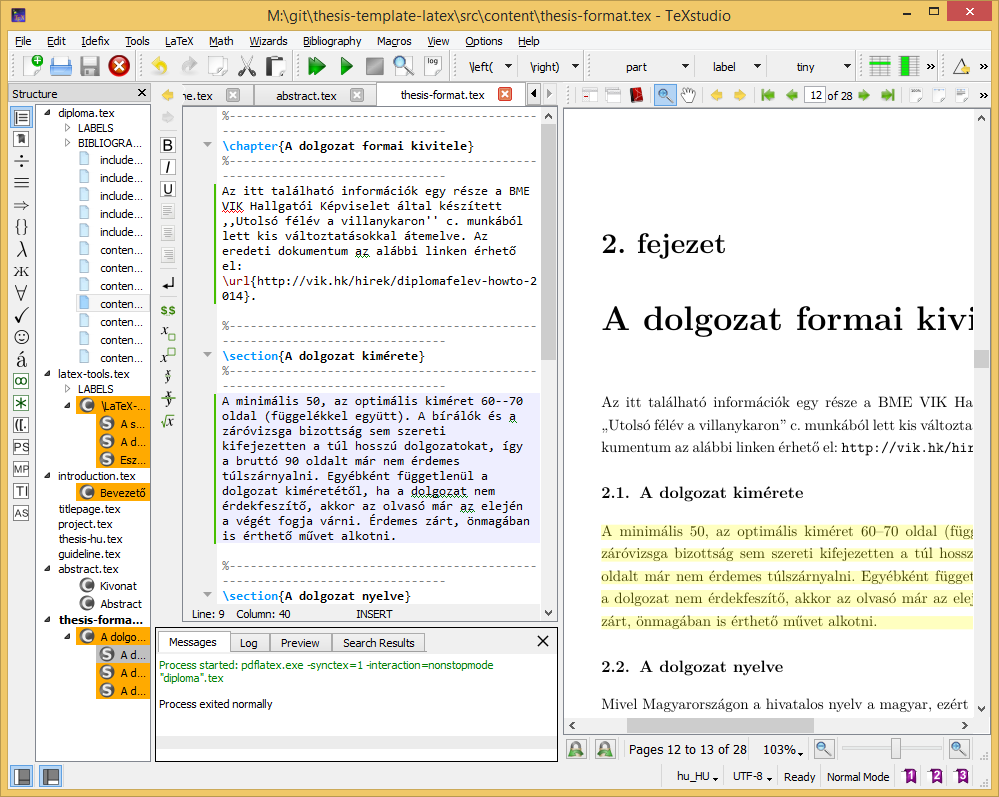
\includegraphics[width=150mm, keepaspectratio]{figures/TeXstudio.png}
\caption{A TeXstudio \LaTeX-szerkesztő.} 
\end{figure}

%----------------------------------------------------------------------------
\clearpage\section{Válasz az ,,Élet, a világmindenség, meg minden'' kérdésére}
%----------------------------------------------------------------------------
A Pitagorasz-tételből levezetve
\begin{align}
c^2=a^2+b^2=42.
\end{align}
A Faraday-indukciós törvényből levezetve
\begin{align}
\rot E=-\frac{dB}{dt}\hspace{1cm}\longrightarrow \hspace{1cm}
U_i=\oint\limits_\mathbf{L}{\mathbf{E}\mathbf{dl}}=-\frac{d}{dt}\int\limits_A{\mathbf{B}\mathbf{da}}=42.
\end{align}


%\label{page:last}
\end{document}
